\documentclass[11pt]{article}

\usepackage[margin=1in]{geometry}
\usepackage{amsmath,amssymb}
\usepackage{booktabs}
\usepackage{graphicx}
\usepackage{tikz}
\usepackage{hyperref}
\usetikzlibrary{arrows.meta,positioning}

\newcommand{\ConvTT}{\mathrm{Conv}_{3\times 3}}

\title{Spectral-Local Residual Networks for Wave Inverse Problems}
\author{}
\date{\today}

\begin{document}
\maketitle

\begin{abstract}
Wave inverse reconstruction requires both a training signal that respects known
measurement physics and an architecture that can map globally coupled
measurements into localized real-space structure. We study these two factors on
synthetic coherent diffractive imaging (CDI). Paired objective controls show
that direct supervised object-space training is insufficient under this CDI
protocol where controls are available: it can give poor or unbalanced
amplitude--phase reconstructions relative to training through the known
diffraction model. We introduce SRU-Net, a spectral-local residual U-Net that
combines truncated Fourier mixing, local convolutional processing, residual
refinement, and convolutional decoding. Under the same CDI physics-consistency
objective, SRU-Net gives the strongest amplitude-side reconstruction among the
tested CNN, FNO, FFNO-local proxy, U-NO, and SRU-Net rows, while U-NO gives the
lowest phase MAE/MSE and SRU-Net gives the strongest phase SSIM. Ablations show
that performance depends not only on spectral capacity, but on where spectral
mixing is placed relative to local paths, residual bottlenecks, and decoder-side
synthesis. We additionally report bounded secondary evidence on Born--Rytov
diffraction tomography inverse scattering and PDEBench compressible
Navier--Stokes. These experiments test transfer and cross-domain context; the
primary claim remains physics-consistent wave inverse reconstruction on CDI.
\end{abstract}

\section{Introduction}

Problems such as phase retrieval, inverse scattering, and forward PDE prediction
combine long-range coupling with localized structure. In lensless computed
imaging, each detector measurement depends on the target object and probe
interaction through global wave propagation, while the reconstruction is a
real-space object with localized amplitude and phase structure. In fluid
dynamics, large-scale coherent dynamics coexist with localized features such as
shocks and vortices. Across these settings, useful learned models must propagate
information globally without erasing localized spatial structure.

Classical forward solvers often require fine discretization, while inverse wave
reconstruction commonly relies on iterative physics-based reconstruction or
projection algorithms. These techniques can be computationally expensive.
Standard computer vision architectures adapted to physics-prediction tasks
provide fast approximate solutions, but their accuracy is limited in domains
with prominent scale mixing. The accuracy gap reflects a specific architectural
mismatch: architectures that are efficient on natural images, such as CNNs,
process local spatial neighborhoods well but lack direct global receptive fields
for long-range physical interactions.

Fourier neural operator (FNO) networks address the opposite side of this
tradeoff. They are effective models for continuous physical systems because
spectral layers provide global mixing \cite{fno}. However, FNO-style models
retain a finite set of Fourier modes, and this truncation can bias predictions
toward lower-frequency structure and weaken sharp localized features. Recent
extensions mitigate this limitation by coupling global Fourier layers with local
or multiscale operators \cite{ufno,localno}. These convolutional, U-Net, or
localized-kernel branches provide a complementary inductive bias for fine-scale
structure while preserving long-range mixing. Such hybrids improve some PDE
benchmarks, but they are not uniformly better than strong spectral-only
architectures such as the factorized Fourier neural operator \cite{ffno}. We
focus on convolutional and spectral inductive biases; attention-based operators
such as Galerkin Transformer and related attention-operator hybrids are a
parallel design axis outside the scope of this study.

Coherent diffractive imaging (CDI) is our primary test case because it stresses
both sides of the global-local problem. Diffraction measurements are globally
coupled by the wave forward model, while the desired output is a localized
complex object. The inverse map must therefore interpret measurement-domain
structure across the full detector field and synthesize a sharp real-space
reconstruction. Our experiments show that FNO-based architectures that are
strong baselines for forward physical prediction can struggle to synthesize
high-quality real-space images from diffraction measurements, although they
still improve over purely convolutional models in several comparisons.

For CDI, the training objective is as important as the architecture. We do not
propose a new CDI loss; instead, we use the established PtychoPINN-style
physics-consistency objective, in which a predicted object is passed through
known real-space consistency and diffraction operators and the loss is applied
in measurement space \cite{hoidn2023physics}. This objective is not an
incidental implementation detail in our experiments. Supervised-only controls
show meaningfully worse aggregate reconstruction quality than the corresponding
+PINN rows across the reported model classes, with the clearest gaps in
amplitude reconstruction. We therefore use the same physics-consistency
objective for the main CDI architecture comparison and ask which network works
best once the standard CDI physics constraint is imposed.

We introduce SRU-Net, a spectral-convolutional architecture for wave inverse
reconstruction. Each encoder block combines a truncated Fourier mixing branch
with a local convolutional branch inside a residual update. The Fourier branch
lets the model aggregate information across the full measurement field, while
the convolutional branch preserves grid-aligned local features. A residual
bottleneck refines the mixed representation at reduced spatial resolution, and a
convolutional decoder synthesizes the real-space output. The architecture is
designed to separate the inverse-mapping role of global spectral mixing from the
image-synthesis role of local convolutional refinement.

Our contributions are threefold. \emph{First}, we introduce SRU-Net, a
spectral-local residual U-Net that combines Fourier-style global mixing with
convolutional local spatial processing inside a residual encoder--bottleneck--decoder
architecture for wave inverse reconstruction. \emph{Second}, on a synthetic CDI
benchmark trained with the PtychoPINN-style physics-consistency objective --
which we show is required for any of the reported architectures to reach
competitive reconstruction quality -- SRU-Net outperforms matched CNN, FNO,
FFNO-local proxy, and U-NO baselines. \emph{Third}, architecture ablations show
that this gain depends on the \emph{placement} of spectral mixing inside the
reconstruction network rather than on spectral capacity alone: replacing the
residual bottleneck with FFNO-style spectral blocks, or weakening the
convolutional decoder, regresses relative to the reference SRU-Net.

The experiments follow this hierarchy. The primary CDI benchmark compares
SRU-Net with CNN, FNO, FFNO-local proxy, and U-NO baselines under the same
physics-consistency objective, while supervised-only controls and architecture
ablations separate the effects of training objective and model design. Born--Rytov
diffraction tomography provides a second inverse-wave transfer setting, where
SRU-Net is compared with a model-based Born inverse and an FFNO-local proxy
under a supervised-plus-Born objective. PDEBench compressible Navier--Stokes
provides cross-domain context: SRU-Net improves over FNO and U-Net under the
matched capped condition used here, while FFNO remains the lowest-error CNS
model.

% Fallback full-field amplitude/phase version retained for quick restoration.
% \begin{figure}[t]
% \centering
% 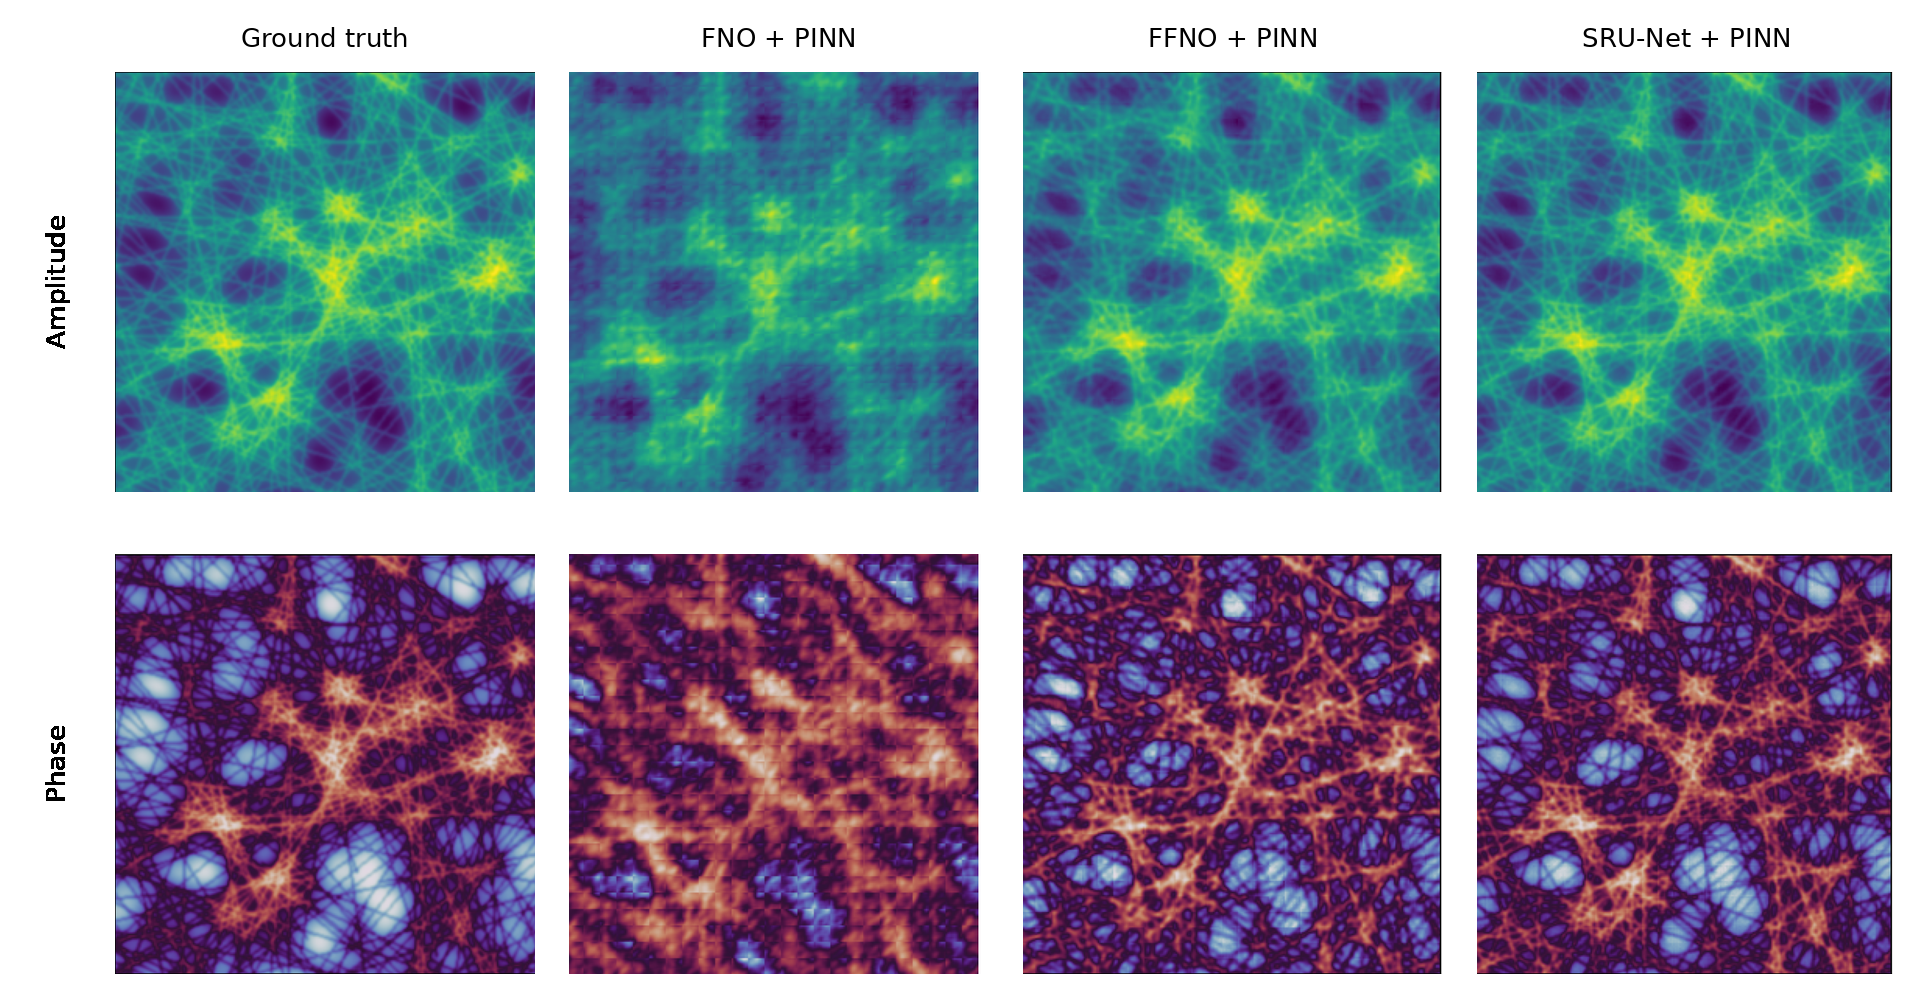
\includegraphics[width=\linewidth]{figures/cdi_synthetic_line_pattern_srunet_fno_ffno.png}
% \caption{\textbf{CDI reconstruction comparison on synthetically-generated diffraction data.} The
% comparison shows ground truth, FNO+PINN, FFNO+PINN, and SRU-Net+PINN under the
% same $N=128$ diffraction data protocol. ``+PINN'' indicates training through
% the CDI physics-consistency loss defined in the introduction.}
% \label{fig:cdi_main_qualitative_full_field_fallback}
% \end{figure}
%
% Alternate contrast-normalized phase-only version. Use only if the caption
% states that each panel is scaled independently and colors are not comparable
% across panels.
% \begin{figure}[t]
% \centering
% 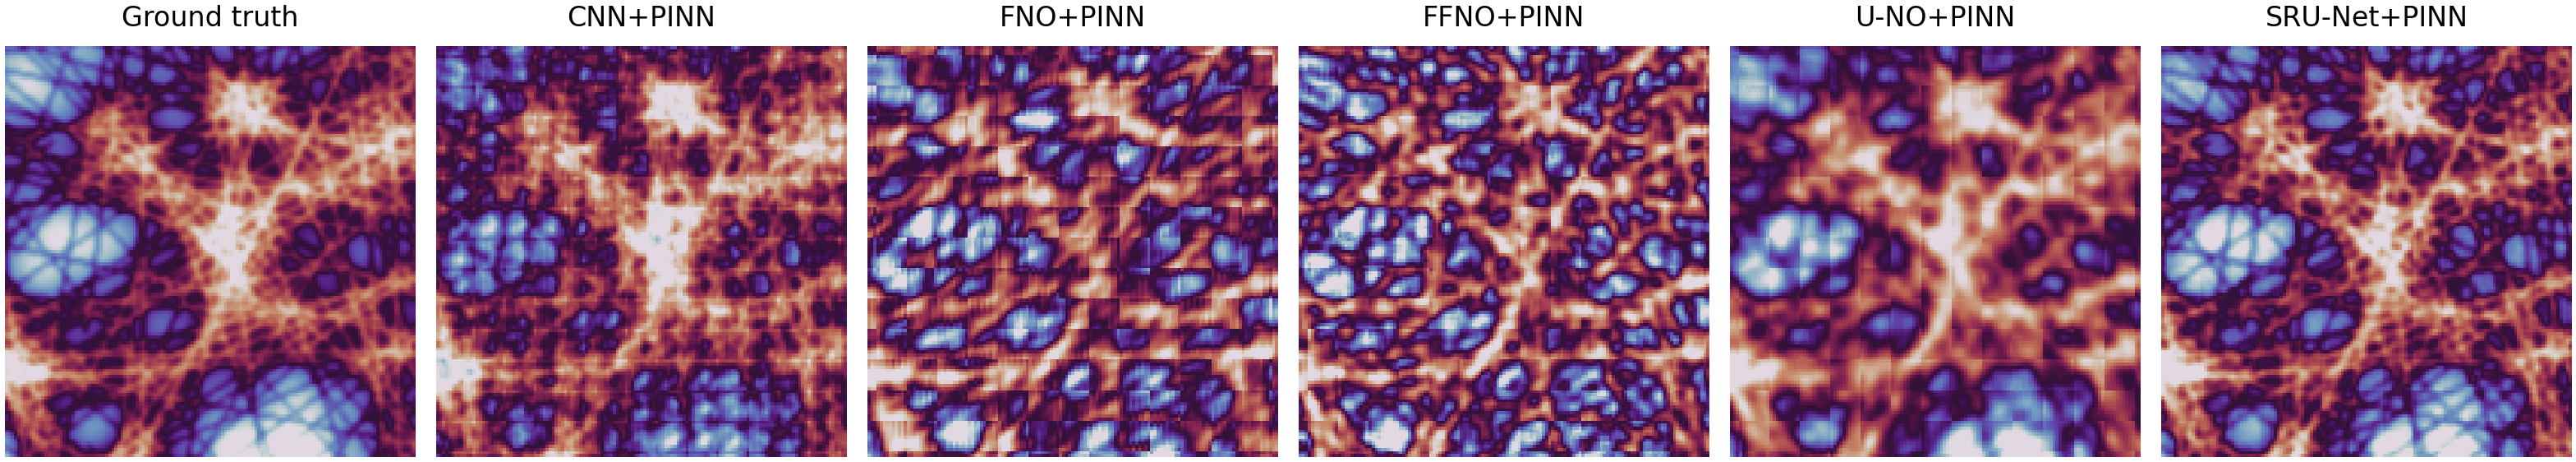
\includegraphics[width=\linewidth]{figures/cdi_lines128_phase_zoom_cnn_fno_ffno_uno_srunet_per_panel_scaled.png}
% \caption{\textbf{Contrast-normalized phase reconstruction comparison.} Each
% panel uses an independent 1st--99th percentile phase scale after global phase
% alignment, so colors reveal within-panel structure but are not directly
% comparable across models.}
% \label{fig:cdi_main_qualitative_per_panel_scaled}
% \end{figure}

\section{Related Work}

\subsection{Operator learning and spectral-local architectures}

Neural operators learn mappings between fields and are widely used for
scientific machine learning. Fourier neural operators (FNOs) apply global
spectral convolutions to represent solution operators for parametric PDEs
\cite{fno}. Factorized Fourier neural operators (FFNOs) make this
parameterization deeper and more efficient by factorizing Fourier transforms,
sharing kernel integral operators across layers, and using residual temporal
updates \cite{ffno}. Their global receptive field is attractive for wave
propagation, diffraction, and fluid dynamics, where distant regions of a field
are coupled by the governing physics. PDEBench provides a controlled setting for
evaluating such models on forward physical prediction tasks, including
compressible Navier--Stokes dynamics \cite{pdebench}.

Pure spectral models provide direct global coupling, but Fourier-mode
truncation can bias predictions toward smoother, lower-frequency structure.
This is problematic when the target contains sharp local features, such as
object boundaries in inverse imaging or high-gradient structures in flow.
Spectral-local architectures address this limitation by combining Fourier
layers with convolutional, U-Net, or localized-kernel branches
\cite{ufno,localno}. These models motivate the SRU-Net design, but they do not
settle which architectural components are needed for physics-consistent wave
inverse reconstruction.

\subsection{Physics-constrained wave inverse reconstruction}

Hoidn, Mishra, and Mehta introduced PtychoPINN for unsupervised scanning-CDI
reconstruction \cite{hoidn2023physics}. The method learns an inverse map from
diffraction data to a complex real-space object, then trains it after passing
the predicted object through known coherent diffractive imaging physics:
overlap-based real-space consistency, the probe interaction, and far-field
diffraction. The loss is applied in measurement space, so the network is
optimized against the measured diffraction statistics rather than only against
paired object targets.

This paper uses that physics-constrained formulation as the primary CDI
training setting. The measurement-consistency objective is not introduced here
as a new CDI forward model. Instead, we use paired objective controls to test
whether direct supervised object-space training is sufficient under our
synthetic CDI protocol. We then ask which architecture works best once the
prediction is trained through the known diffraction physics.

\subsection{This paper's position}

SRU-Net follows the spectral-local design principle in a network built for wave
inverse reconstruction. It combines spectral-local encoder blocks, residual
bottleneck refinement, and decoder-side upsampling inside a reconstruction
architecture trained through a physics-consistency loss. The CDI experiments are
the primary test because they evaluate both central factors: objective and
architecture. BRDT tests whether the same reconstruction bias transfers to a
second wave inverse problem, and PDEBench CNS tests the architecture in a
supervised forward-prediction setting where FFNO remains a strong reference
baseline.

\section{Methods}

\subsection{Task-agnostic network formulation}

Let $x$ denote the task input and $y$ the target field or reconstruction. We
write the learned network as
\begin{equation}
  \hat{y} = G_{\theta}(x).
\end{equation}
For CDI, $x$ is a stack of diffraction measurements and $\hat{y}$ is a complex
object-patch representation, meaning local crops of the reconstructed complex
object represented by real and imaginary channels. For BRDT, $x$ is a
Born-derived image-space initialization and $\hat{y}$ is the recovered
scattering potential. For PDEBench CNS, $x$ is a temporal history of physical
fields and $\hat{y}$ is the predicted next state. The tasks use
different input representations and objective functions, but share the same
architectural principle:
$G_{\theta}$ combines global spectral mixing with local convolutional feature
recovery.

We decompose the network as
\begin{equation}
  G_{\theta} = D_{\theta} \circ B_{\theta} \circ E_{\theta},
\end{equation}
where $E_{\theta}$ is the spectral-local encoder, $B_{\theta}$ is a ResNet
bottleneck at reduced spatial resolution, and $D_{\theta}$ is a convolutional
upsampling decoder.

We use subscripts to distinguish architectural positions rather than tensor
dimensions. The index $\ell$ denotes the encoder block that maps
$z_{\ell}$ to $z_{\ell+1}$; $j$ indexes the six residual bottleneck blocks;
$s$ indexes resolution levels used for encoder-decoder skip connections; and
$k$ indexes Fourier modes. The retained Fourier-mode set is $K$, with
$m=|K|$ in the architecture diagram. Superscripts such as $B_j^{\times 6}$
denote repeated blocks rather than exponentiation. Task subscripts such as
${\rm CDI}$ and ${\rm CNS}$ label task-specific outputs.

\subsection{Spectral-local encoding}

For a feature tensor $z_{\ell}$, a spectral-local encoder block has the form
\begin{equation}
z_{\ell+1}
= \sigma\left(
L_{\ell} z_{\ell}
+ \mathcal{F}^{-1}
\left[
R_{\ell}(k)\,\mathcal{T}_{K}\left(\mathcal{F}(z_{\ell})\right)(k)
\right]
\right),
\end{equation}
where $L_{\ell}$ is a learned local convolutional map, $\mathcal{F}$ is the 2D
Fourier transform, $\mathcal{T}_{K}$ retains a fixed set of Fourier modes,
$R_{\ell}(k)$ is a learned complex spectral mixing tensor over retained modes,
and $\sigma$ is the GELU nonlinearity used in the implemented SRU-Net. In
residual form, this can be written as
\begin{equation}
z_{\ell+1}
= z_{\ell} + \sigma\left(L_{\ell} z_{\ell} + S_{\ell} z_{\ell}\right),
\end{equation}
with $S_{\ell}$ denoting the truncated spectral operator. The local path
preserves high-frequency and edge-like information that may be weakened by
spectral truncation, while the spectral path provides global coupling.

\subsection{Spectral-convolutional residual architecture}

The implemented SRU-Net consists of an initial convolution, four spectral-local
encoder blocks, two downsampling stages, a
six-block residual bottleneck at $N/4$ spatial resolution, and a convolutional
upsampling decoder. Figure~\ref{fig:srunet_architecture} summarizes the data flow, and
Table~\ref{tab:architecture_summary} lists the architectural choices that
determine the shape of the model.

In the architecture diagram, $\phi_0$ is the initial channel projection, $E_0$
through $E_3$ are encoder blocks, $B_j$ denotes a residual bottleneck block, and
$U_1,U_2$ are decoder upsampling stages. The spatial resolution is denoted by
$N$, $C_{\rm in}$ is the task-specific input channel count, $m$ is the number of
retained Fourier modes, and $e_s,d_s$ are encoder and decoder features at scale
$s$. The skip projection $P_s$ maps encoder features into the decoder channel
space before additive fusion.
Within encoder block $E_\ell$, $z_\ell$ is the input feature tensor,
$S_\ell=\mathcal F^{-1}R_\ell\mathcal T_K\mathcal F$ is the truncated spectral
operator, $L_\ell$ is the local convolutional path, and $\sigma$ is GELU. Here
$\mathcal F$ is the Fourier transform, $\mathcal T_K$ keeps the retained modes,
and $R_\ell$ mixes those modes. Within bottleneck block
$B_j$, $u_j$ is the bottleneck feature tensor,
$R_j=\ConvTT\cdot\mathrm{InstNorm}\cdot\mathrm{GELU}
\cdot\ConvTT\cdot\mathrm{InstNorm}$ is applied before the
residual addition, and $\alpha_j$ is its learned residual scale; the centered
dot lists operations in left-to-right order. Here $\ConvTT$ denotes a
3-by-3 convolution. Within decoder stage $D_s$, $U_s$ upsamples the coarser
decoder state and $P_s$ projects the matching encoder feature before fusion.

\begin{figure}[t]
\centering
\resizebox{\linewidth}{!}{%
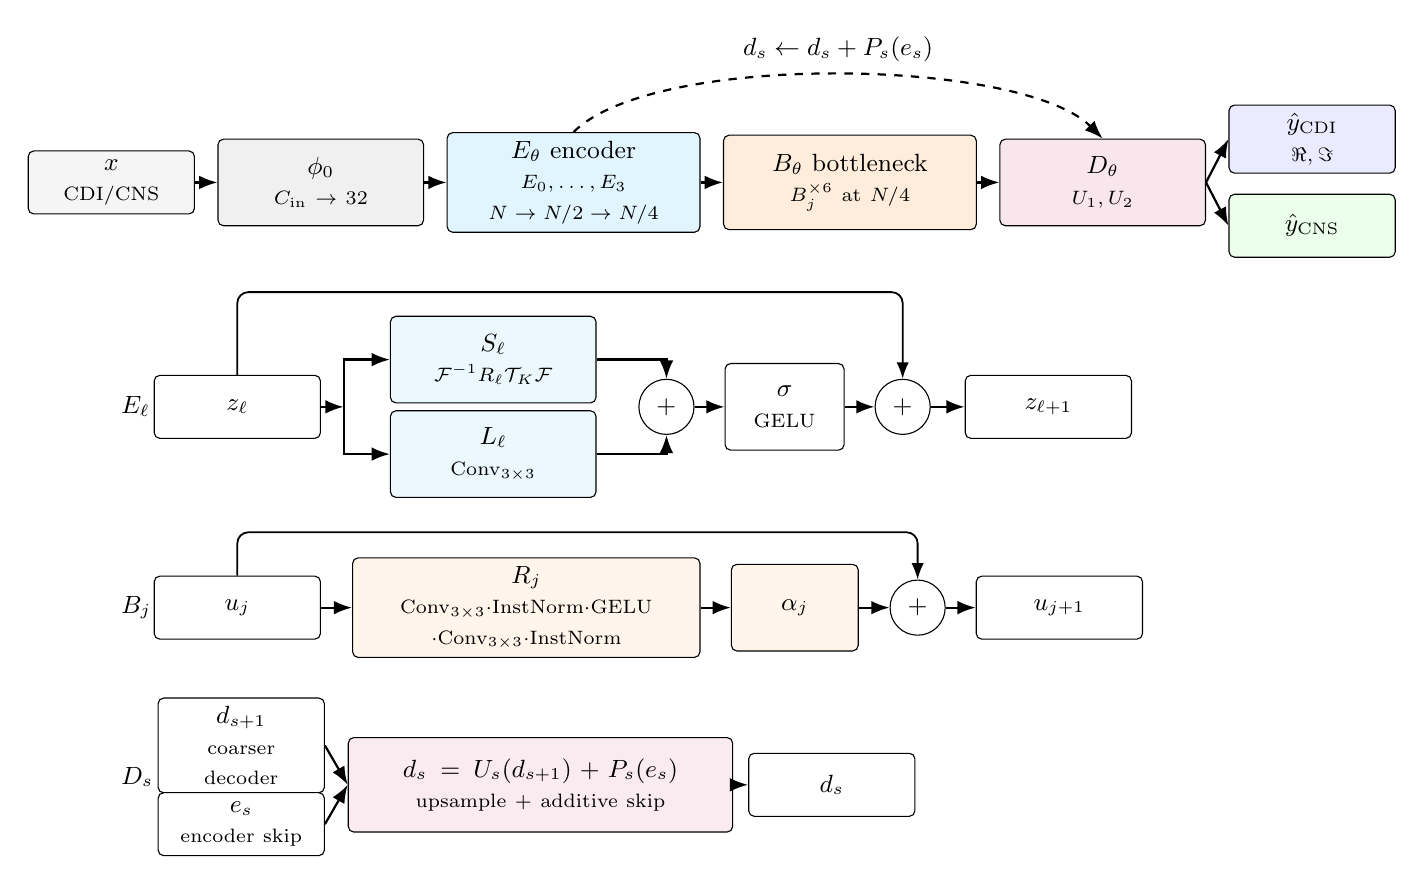
\begin{tikzpicture}[
  >=Latex,
  tensor/.style={draw, rounded corners=2pt, align=center, minimum height=8mm, text width=19mm, inner sep=3pt, font=\small},
  block/.style={draw, rounded corners=2pt, align=center, minimum height=11mm, text width=24mm, inner sep=3pt, font=\small},
  wideblock/.style={draw, rounded corners=2pt, align=center, minimum height=12mm, text width=30mm, inner sep=3pt, font=\small},
  op/.style={draw, circle, minimum size=7mm, inner sep=0pt, font=\small},
  formula/.style={draw, rounded corners=2pt, align=center, minimum height=12mm, text width=46mm, inner sep=4pt, font=\small},
  flow/.style={-Latex, line width=0.8pt},
  skip/.style={-Latex, dashed, line width=0.8pt},
  bypass/.style={-Latex, line width=0.65pt}
]
% Row 1: top-level pipeline
\node[tensor, fill=gray!8] (input) at (0,0) {$x$\\{\scriptsize CDI/CNS}};
\node[block, fill=gray!12] (lift) at (2.66,0)
  {$\phi_0$\\{\scriptsize $C_{\rm in}\!\to\!32$}};
\node[wideblock, fill=cyan!12] (encoder) at (5.87,0)
  {$E_\theta$ encoder\\{\scriptsize $E_0,\ldots,E_3$}\\{\scriptsize $N\!\to\!N/2\!\to\!N/4$}};
\node[wideblock, fill=orange!14] (bottleneck) at (9.38,0)
  {$B_\theta$ bottleneck\\{\scriptsize $B_j^{\times 6}$ at $N/4$}};
\node[block, fill=purple!10] (decoder) at (12.59,0)
  {$D_\theta$\\{\scriptsize $U_1,U_2$}};
\node[tensor, fill=blue!8] (cdiout) at (15.25,0.55)
  {$\hat y_{\rm CDI}$\\{\scriptsize $\Re,\Im$}};
\node[tensor, fill=green!8] (cnsout) at (15.25,-0.55)
  {$\hat y_{\rm CNS}$};

\draw[flow] (input) -- (lift);
\draw[flow] (lift) -- (encoder);
\draw[flow] (encoder) -- (bottleneck);
\draw[flow] (bottleneck) -- (decoder);
\draw[flow] (decoder.east) -- (cdiout.west);
\draw[flow] (decoder.east) -- (cnsout.west);

% Flatter skip arc
\draw[skip] (encoder.north) to[out=45,in=135,looseness=0.55]
  node[above=1pt, font=\small] {$d_s \leftarrow d_s + P_s(e_s)$}
  (decoder.north);

% Row 2: Encoder block detail (zoom of E_theta)
\node[font=\small\bfseries, anchor=west] at (0,-2.85) {$E_\ell$};
\node[tensor, fill=white] (rx) at (1.6,-2.85) {$z_\ell$};
\coordinate (rxbranch) at (2.95,-2.85);
\node[block, fill=cyan!8] (spec) at (4.85,-2.25)
  {$S_\ell$\\{\scriptsize $\mathcal F^{-1}R_\ell\mathcal T_K\mathcal F$}};
\node[block, fill=cyan!8] (conv) at (4.85,-3.45)
  {$L_\ell$\\{\scriptsize $\ConvTT$}};
\node[op] (sum1) at (7.05,-2.85) {$+$};
\node[block, fill=white, text width=13mm] (gelu) at (8.55,-2.85)
  {$\sigma$\\{\scriptsize GELU}};
\node[op] (sum2) at (10.05,-2.85) {$+$};
\node[tensor, fill=white] (ry) at (11.9,-2.85) {$z_{\ell+1}$};

\draw[flow] (rx.east) -- (rxbranch);
\draw[flow] (rxbranch) |- (spec.west);
\draw[flow] (rxbranch) |- (conv.west);
\draw[flow] (spec.east) -| (sum1.north);
\draw[flow] (conv.east) -| (sum1.south);
\draw[flow] (sum1.east) -- (gelu.west);
\draw[flow] (gelu.east) -- (sum2.west);
\draw[flow] (sum2.east) -- (ry.west);
\draw[bypass, rounded corners=4pt]
  (rx.north) -- ++(0,1.05) -| (sum2.north);

% Row 3: Bottleneck block detail (zoom of B_theta)
\node[font=\small\bfseries, anchor=west] at (0,-5.4) {$B_j$};
\node[tensor, fill=white] (bx) at (1.6,-5.4) {$u_j$};
\node[wideblock, fill=orange!8, text width=42mm] (rescore) at (5.27,-5.4)
  {$R_j$\\{\scriptsize $\ConvTT\cdot$InstNorm$\cdot$GELU}\\{\scriptsize $\cdot\ConvTT\cdot$InstNorm}};
\node[block, fill=orange!8, text width=14mm] (scale) at (8.68,-5.4) {$\alpha_j$};
\node[op] (bsum) at (10.24,-5.4) {$+$};
\node[tensor, fill=white] (by) at (12.04,-5.4) {$u_{j+1}$};

\draw[flow] (bx) -- (rescore);
\draw[flow] (rescore) -- (scale);
\draw[flow] (scale) -- (bsum);
\draw[flow] (bsum) -- (by);
\draw[bypass, rounded corners=4pt]
  (bx.north) -- ++(0,0.55) -| (bsum.north);

% Row 4: Decoder stage detail (zoom of D_theta)
\node[font=\small\bfseries, anchor=west] at (0,-7.55) {$D_s$};
\node[tensor, fill=white] (din) at (1.65,-7.15) {$d_{s+1}$\\{\scriptsize coarser decoder}};
\node[tensor, fill=white] (eskip) at (1.65,-8.15) {$e_s$\\{\scriptsize encoder skip}};
\node[formula, fill=purple!8] (dformula) at (5.45,-7.65)
  {$d_s = U_s(d_{s+1}) + P_s(e_s)$\\{\scriptsize upsample + additive skip}};
\node[tensor, fill=white] (dout) at (9.15,-7.65) {$d_s$};

\draw[flow] (din.east) -- (dformula.west);
\draw[flow] (eskip.east) -- (dformula.west);
\draw[flow] (dformula.east) -- (dout.west);
\end{tikzpicture}%
}
\caption{\textbf{SRU-Net combines spectral global mixing with local spatial
processing.} Top: $x$ is the task input, $\phi_0$ projects $C_{\rm in}$ input
channels to width 32, $E_\theta$ is the encoder over resolutions
$N\!\to\!N/2\!\to\!N/4$, $B_\theta$ is the
six-block bottleneck, $D_\theta$ is the decoder, and
$\hat y_{\rm CDI},\hat y_{\rm CNS}$ are task-specific outputs. Middle:
encoder block $E_\ell$ maps $z_\ell$ to $z_{\ell+1}$ using spectral path
$S_\ell=\mathcal F^{-1}R_\ell\mathcal T_K\mathcal F$, local convolution path
$L_\ell$, GELU nonlinearity $\sigma$, and a residual bypass. The bottleneck
detail shows that
bottleneck block $B_j$ maps $u_j$ to $u_{j+1}$ by applying $R_j$, then scaling
it by $\alpha_j$ before adding it to the bypassed input. The $R_j$ box uses
centered dots to list left-to-right sequential application; $\ConvTT$ denotes a
3-by-3 convolution and InstNorm denotes instance normalization. The decoder
detail writes the stage directly as
$d_s = U_s(d_{s+1}) + P_s(e_s)$, where $U_s$ upsamples the coarser decoder
feature and $P_s$ projects the encoder skip feature before additive fusion.}
\label{fig:srunet_architecture}
\end{figure}

% table_metadata: cap_size=not_applicable; table_type=architecture_summary
\begin{table}[h]
\centering
\small
\caption{\textbf{SRU-Net architecture summary.} The same architecture is used
for CDI reconstruction and CNS field prediction, with task-specific input
representations, output variables, and objective functions.}
\label{tab:architecture_summary}
\begin{tabular}{p{0.22\linewidth}p{0.68\linewidth}}
\toprule
Component & Implementation details \\
\midrule
Input representation & CDI uses grouped object-patch channels and
returns complex real/imaginary patches. CNS uses real-valued field histories as
input and predicts the next density, velocity, and pressure fields. In both
settings, the first convolution maps the input to width 32. \\
Encoder & Four spectral-local blocks. Each block adds a learned Fourier-mode
mixing branch and a reflected-padding $3\times 3$ convolution branch inside an
outer residual update; the branch sum is passed through GELU before the outer
residual addition. The retained-mode count $m$ is a configurable parameter; the
reported base setting uses $m=12$ unless otherwise stated. The encoder
downsamples after the first two blocks, giving $N\to N/2\to N/4$ and widths
32, 64, and 128. \\
Bottleneck & Six constant-resolution residual blocks at $N/4$. Each block uses
a reflected-padding $3\times 3$ convolution, instance normalization, GELU, a
second reflected-padding $3\times 3$ convolution, instance normalization, and a
learned residual scale. The spectral-residual variant replaces this local
bottleneck with residual blocks that add a shared factorized spectral branch. \\
Decoder and skips & The CDI path uses two transposed-convolution upsampling
stages. The selected CNS row uses two pixel-shuffle upsampling stages and
projected additive encoder-decoder skips from the $N/2$ and $N$ encoder
resolutions. \\
Output and loss & CDI predicts real/imaginary complex patches and trains through
the coherent diffractive imaging consistency and diffraction operators. BRDT
predicts a real scattering potential and trains with supervised object loss
plus Born consistency. CNS predicts real field channels and trains against the
next physical state. \\
\bottomrule
\end{tabular}
\end{table}

When skip connections are enabled, encoder features $e_s$ are fused into decoder
states $d_s$. For additive fusion,
\begin{equation}
  d_s = U_s(d_{s+1}) + P_s(e_s),
\end{equation}
where $U_s$ upsamples the coarser decoder state and $P_s$ projects the encoder
feature into the decoder channel space. For concatenative fusion,
\begin{equation}
  d_s = P_s\left([U_s(d_{s+1}), e_s]\right).
\end{equation}
The CDI network outputs complex object patches in real/imaginary format. In
BRDT, the same reconstruction architecture outputs a single real scattering
potential. In the PDEBench experiments, the architecture is evaluated on
real-valued physical field histories and next-state targets rather than
diffraction measurements.

\subsection{CDI physics-consistency objective}

For CDI, SRU-Net predicts local complex object patches,
\begin{equation}
  \hat{o} = G_{\theta}(x).
\end{equation}
The prediction is not trained only by comparing $\hat{o}$ to a paired object
target. Instead, it is passed through a real-space consistency operator $F_c$,
which stitches overlapping local patches into a common object canvas and
re-extracts position-consistent patches. The consistent object patches are then
passed through a known diffraction map $F_d$:
\begin{equation}
  \hat{x}
  = F_d\left(F_c(\hat{o}; r); P\right),
\end{equation}
where $r$ denotes scan positions and $P$ is the probe. The CDI objective is
defined in measurement space:
\begin{equation}
  \mathcal{L}_{\mathrm{CDI}}
  = \mathcal{D}\left(x, F_d(F_c(G_{\theta}(x); r); P)\right)
  + \lambda R(G_{\theta}(x)).
\end{equation}
Here $\mathcal{D}$ is the experiment-specific measurement loss, such as Poisson
negative log likelihood or amplitude/intensity reconstruction error, and $R$
denotes optional reconstruction regularization. This is the
physics-consistency objective used in the CDI architecture comparison and in the
paired objective controls.

\subsection{CDI supervised objective controls}

To isolate the role of the training signal, we also train supervised
object-space controls for architectures where paired rows are available. These
controls use the same input data, architecture family, optimizer, training
budget, and evaluation metrics as their physics-informed counterparts, but the
loss is applied directly to the predicted object representation rather than
after the CDI forward model. We report these rows only as objective controls;
the main architecture comparison is made under the shared physics-consistency
objective.

The supervised objective has the form
\begin{equation}
  \mathcal{L}_{\mathrm{sup}}
  =
  \mathcal{D}_{\mathrm{obj}}\left(G_{\theta}(x), y\right),
\end{equation}
where $y$ is the paired object target and
$\mathcal{D}_{\mathrm{obj}}$ is the object-space reconstruction loss used by
the corresponding control run. Metrics are computed after the same evaluation
alignment and post-processing used for physics-informed rows.

\subsection{Born--Rytov diffraction tomography}

We also evaluate SRU-Net on a Born--Rytov diffraction tomography (BRDT)
inverse-scattering task. The target is the physical scattering potential
\begin{equation}
  q(x,z) = k_m^2\left[\left(\frac{n(x,z)}{n_m}\right)^2 - 1\right],
\end{equation}
where $n(x,z)$ is the refractive-index field, $n_m$ is the background medium
index, and $k_m$ is the in-medium wavenumber. Under the first Born
approximation, each incident plane wave produces a scattered field whose
far-field samples are linear measurements of the Fourier transform of $q$ on
the corresponding Ewald arc. We write this discrete forward map as
\begin{equation}
  s = \mathcal{B}(q),
\end{equation}
where $s \in \mathbb{R}^{A \times D \times 2}$ is the complex sinogram over
illumination angles and detector frequencies, represented by real and imaginary
channels.

The BRDT network input is a Born-derived image-space initialization
$x_{\mathrm{BRDT}}$ computed from the measured sinogram. The model predicts a
single-channel scattering potential,
\begin{equation}
  \hat{q}_{\theta} = G_{\theta}(x_{\mathrm{BRDT}}).
\end{equation}
All neural rows use the same input representation and the same differentiable
Born forward operator during training.

The BRDT objective combines supervised reconstruction with measurement-space
Born consistency:
\begin{align}
  \mathcal{L}_{\mathrm{BRDT}}
  &=
  \lambda_{\mathrm{img}}
  \left\|\hat{q}_{\theta}^{\,\mathrm{norm}} - q^{\mathrm{norm}}\right\|_1
  +
  \lambda_{\mathrm{abs}}
  \left\|\mathcal{B}(\hat{q}_{\theta}) - s\right\|_1 \nonumber \\
  &\quad+
  \lambda_{\mathrm{rel}}
  \frac{
    \left\|\mathcal{B}(\hat{q}_{\theta}) - s\right\|_2
  }{
    \left\|s\right\|_2 + \epsilon
  }
  +
  \lambda_{\mathrm{tv}}\,\mathrm{TV}(\hat{q}_{\theta})
  +
  \lambda_{\mathrm{pos}}
  \left\|\min(\hat{q}_{\theta},0)\right\|_2^2 .
\end{align}
The image loss is computed in the normalized target space used by the model.
Before applying the Born operator, predictions are converted back to physical
$q$ units using training-set normalization statistics. This prevents the
measurement-consistency term from being evaluated on normalized, dimensionless
outputs. We use $\lambda_{\mathrm{img}}=1$,
$\lambda_{\mathrm{abs}}=0.1$, $\lambda_{\mathrm{rel}}=0.1$,
$\lambda_{\mathrm{tv}}=10^{-5}$, and
$\lambda_{\mathrm{pos}}=10^{-4}$.

\subsection{PDEBench CNS supervised prediction}

For the CNS benchmark, the same architecture is evaluated as a supervised
forward predictor. Let
\begin{equation}
  u_t = [\rho_t, v_{x,t}, v_{y,t}, p_t]
\end{equation}
be the density, velocity, and pressure state. Given a history length $h$, the
input is
\begin{equation}
  x_t = [u_{t-h}, \ldots, u_{t-1}],
\end{equation}
and the model predicts
\begin{equation}
  \hat{u}_t = G_{\theta}(x_t).
\end{equation}
The training objective is mean-squared error on normalized physical fields:
\begin{equation}
  \mathcal{L}_{\mathrm{CNS}}
  = \left\|\hat{u}_t - u_t\right\|_2^2.
\end{equation}
Evaluation is performed after denormalization and reports root mean squared
error (RMSE), normalized RMSE (nRMSE), relative $L_2$, and Fourier-band RMSE
over low, mid, and high radial-frequency bands. The
high-frequency metric is included because shocks and localized vortical features
are precisely where global spectral models may lose detail.

\section{Experiments}

We organize the experiments around one primary benchmark and two bounded
supporting checks. The primary benchmark is synthetic CDI, where we evaluate the
two central factors of the paper: supervised versus physics-consistency training
and architecture choice under a shared physics-consistency objective. BRDT is a
secondary wave inverse problem used to test transfer of the reconstruction
architecture. PDEBench CNS is a secondary supervised forward-prediction setting
used to contextualize the architecture against operator-learning baselines. The
paper's main claim is therefore not full PDEBench state-of-the-art performance,
but physics-consistent wave inverse reconstruction on CDI.

\paragraph{Baseline naming.}
Rows labeled FFNO-local proxy use an FFNO-style spectral stack followed by local
CNN refinement. They are reported as implementation-specific spectral-local
FFNO variants, not as canonical pure-FFNO baselines. We therefore avoid using
these rows to make pure-FFNO claims; corrected no-refiner FFNO rows are required
for that comparison.

\subsection{Primary CDI benchmark}

The primary benchmark is a 128-by-128 CDI reconstruction task with
synthetically generated diffraction data. Each sample is generated from sharp
line-like objects, a known probe, and simulated far-field diffraction
measurements. The network predicts complex object patches, the CDI consistency
and diffraction operators map the prediction back to detector space, and
reconstruction quality is measured against held-out object amplitude and phase.

The CDI experiments are organized in two stages. First, we compare direct
supervised object-space training with physics-consistency training for
architectures where paired controls are available. This tests whether the
forward-model objective is necessary under the synthetic CDI protocol. Second,
we compare CNN, FNO, FFNO-local proxy, U-NO, and SRU-Net-style architectures
under the shared CDI physics-consistency objective. This tests which network
architecture works best once the training signal is fixed.

The synthetic CDI comparison uses $N=128$ object grids, two training objects, two
held-out test objects, $10^9$ photons per exposure, 40 training epochs,
learning rate $2\times 10^{-4}$, ReduceLROnPlateau scheduling,
and complex-valued real/imaginary network output. Phase metrics are computed
after the same global alignment procedure for all rows. Appendix
Table~\ref{tab:model_config_by_benchmark} reports the effective configuration
of each reported model row; parameter counts are unique trainable parameters in
the effective prediction model.

\subsection{BRDT inverse-scattering transfer}

The BRDT experiment is a controlled secondary inverse-scattering study. It uses
$128\times128$ scattering-potential fields and simulated complex sinograms from
a differentiable Born forward model with 64 illumination angles and 128
detector samples. We use it to test whether the CDI reconstruction architecture
transfers to a related wave inverse problem; it is not used as a primary
benchmark claim. We train SRU-Net and FFNO for 40 epochs on the same
2048/256/256 train/validation/test split, using Adam with learning rate
$2\times10^{-4}$, batch size 16, seed 42, and ReduceLROnPlateau scheduling.
Both rows use the same Born-derived image initialization as input and the same
supervised-plus-Born-consistency objective defined above.

\subsection{PDEBench CNS transfer}

The secondary benchmark is PDEBench 2D compressible Navier-Stokes at native
$128\times128$ resolution. It stresses the same architectural tradeoff in a
different physical setting: coherent global flow and wave structure must be
predicted while preserving localized shocks, vortices, and high-gradient field
features. It therefore tests whether the SRU-Net architecture
transfers beyond the CDI inverse problem.

The selected CNS data are the official 128-by-128 periodic compressible-flow
training trajectories at Mach number $M=1.0$, shear viscosity
$\eta=0.01$, and bulk viscosity $\zeta=0.01$. The spatial grid has
$\Delta x=\Delta y=1/128=0.0078125$, the temporal spacing is
$\Delta t=0.05$, and the spatial boundary condition is periodic, meaning that
values wrap around at the domain edges as on a torus. Each trajectory contains
the fields density, $v_x$, $v_y$, and pressure on a $128\times128$ grid.
Splits are trajectory-level, normalization is computed from the train split
only, and metrics are evaluated on denormalized predictions.

\section{Results}

We organize the results around the same hierarchy as the experiments. The CDI
results are primary and answer two questions: whether physics-consistency is
needed as a training signal, and which architecture performs best under that
shared objective. The BRDT results provide secondary inverse-scattering
transfer evidence. The CNS results provide secondary cross-domain context for
the architecture in supervised forward prediction.

\subsection{Primary CDI objective controls}

Table~\ref{tab:cdi_lines128_objective_controls} tests whether the
physics-consistency objective is merely a training detail. For architectures
where paired rows are available, direct supervised object-space training gives
poor or unbalanced reconstructions relative to training through the diffraction
model. In particular, supervised rows can improve selected phase-error metrics
while degrading amplitude reconstruction or phase structure, whereas
physics-consistency training gives stronger measurement-consistent amplitude
recovery and phase SSIM.

% table_metadata: task=CDI_lines128; table_type=pinn_vs_supervised_controls; authority=complete_lines128_cdi_benchmark_plus_uno_extension; source=docs/plans/NEURIPS-HYBRID-RESNET-2026/tables/cdi_lines128_objective_comparison.tex; metrics=mae,ssim; paired_models=cnn,ffno,uno
\begin{table}[t]
\centering
\scriptsize
\setlength{\tabcolsep}{2pt}
\caption{\textbf{Synthetic CDI objective controls.}
Each block compares physics-informed and supervised training for the same
architecture where both rows are available. These controls test the training
signal rather than the architecture alone. Lower MAE is better; higher SSIM is
better.}
\label{tab:cdi_lines128_objective_controls}
\begin{tabular}{lrrrr}
\toprule
Objective & Amp MAE & Phase MAE & Amp SSIM & Phase SSIM \\
\midrule
\multicolumn{5}{l}{\textit{FFNO}} \\
\midrule
PINN & \textbf{0.0820} & 0.1380 & \textbf{0.8903} & \textbf{0.9596} \\
Supervised & 0.3515 & \textbf{0.0661} & 0.2650 & 0.9015 \\
\bottomrule
\end{tabular}

\end{table}

\subsection{Primary CDI architecture comparison}

After fixing the training signal to the CDI physics-consistency objective,
architecture still matters. Table~\ref{tab:cdi_lines128_pinn} compares local,
spectral, and spectral-local models under the same $N=128$ line-pattern
protocol. SRU-Net gives the best amplitude-side reconstruction among the
PINN-trained models by MAE, MSE, and SSIM. U-NO gives the lowest phase MAE and
MSE, while SRU-Net gives the strongest phase SSIM. The historical FFNO-local
proxy improves over the CNN and FNO PINN rows but does not match SRU-Net's
amplitude-side reconstruction on this CDI task.

% table_metadata: task=CDI_lines128; table_type=pinn_model_comparison; authority=complete_lines128_cdi_benchmark_plus_uno_extension; source=docs/plans/NEURIPS-HYBRID-RESNET-2026/tables/cdi_lines128_pinn_metrics.tex; metrics=mae,mse,ssim; includes_uno=true
\begin{table}[t]
\centering
\scriptsize
\setlength{\tabcolsep}{2pt}
\caption{\textbf{Synthetic CDI architecture comparison under
physics-consistency training.} All rows use the same $N=128$ line-pattern
protocol and CDI physics-consistency objective. FFNO-local proxy denotes an
FFNO-style spectral stack followed by local CNN refinement and is not a
canonical pure-FFNO baseline.}
\label{tab:cdi_lines128_pinn}
\resizebox{\textwidth}{!}{\begin{tabular}{lrrrrrr}
\toprule
Model & Amp MAE $\downarrow$ & Phase MAE $\downarrow$ & Amp MSE $\downarrow$ & Phase MSE $\downarrow$ & Amp SSIM $\uparrow$ & Phase SSIM $\uparrow$ \\
\midrule
CNN & 0.1232 & 0.7863 & 0.0237 & 1.1843 & 0.7326 & 0.2638 \\
FNO & 0.1248 & 0.1435 & 0.0240 & 0.0323 & 0.7409 & 0.9335 \\
FFNO-local proxy & 0.0628 & 0.0828 & 0.0062 & 0.0109 & 0.9348 & 0.9816 \\
SRU-Net & \textbf{0.0269} & 0.0721 & \textbf{0.0012} & 0.0078 & \textbf{0.9881} & \textbf{0.9947} \\
U-NO & 0.0932 & \textbf{0.0683} & 0.0132 & \textbf{0.0073} & 0.8280 & 0.9569 \\
\bottomrule
\end{tabular}
}
\end{table}

% figure_metadata: task=CDI_lines128; paper_copy=figures/cdi_lines128_phase_zoom_cnn_fno_ffno_uno_srunet.png; visible_columns=gt,pinn,pinn_fno_vanilla,pinn_ffno,pinn_neuralop_uno,pinn_hybrid_resnet; display_channel=phase; crop_fraction=0.5; phase_alignment=global_circular_offset_to_gt_before_wrapping; phase_colormap=twilight; phase_display_scale=gt_crop_min_to_gt_crop_p99_after_alignment; source=.artifacts/work/NEURIPS-HYBRID-RESNET-2026/backlog/2026-04-30-cdi-lines128-uno-table-extension/runs/complete_table_plus_uno_20260504T100347Z/recons
\begin{figure}[t]
\centering
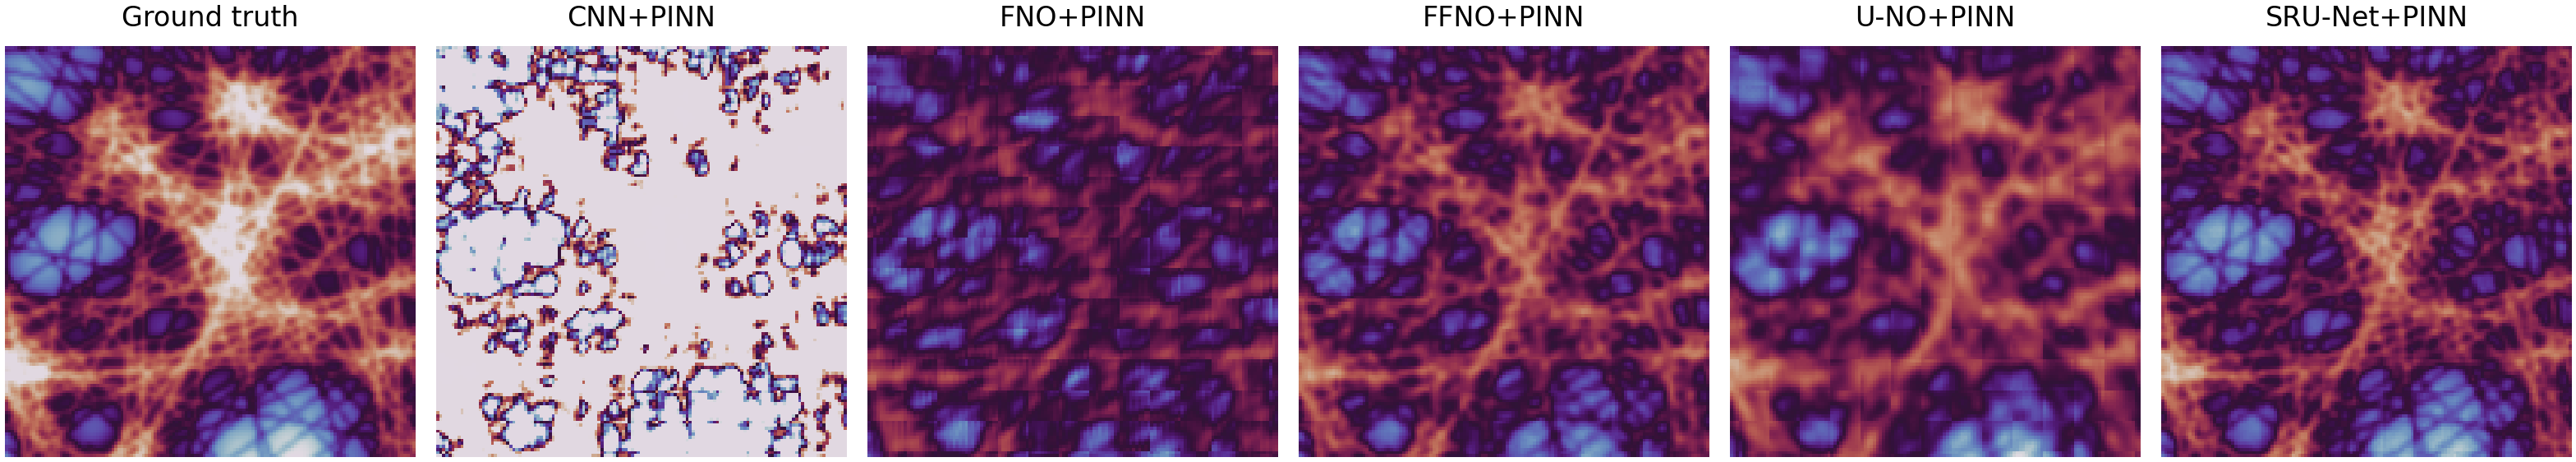
\includegraphics[width=\linewidth]{figures/cdi_lines128_phase_zoom_cnn_fno_ffno_uno_srunet.png}
\caption{\textbf{Phase reconstruction comparison on synthetically generated CDI
data.} The cropped comparison shows ground truth, CNN+PINN, FNO+PINN,
FFNO-local proxy+PINN, U-NO+PINN, and SRU-Net+PINN under the same $N=128$
diffraction protocol. Each prediction is aligned to the ground-truth phase by a
single global circular offset before display.}
\label{fig:cdi_main_qualitative}
\end{figure}

\subsection{CDI architecture ablations}

Table~\ref{tab:cdi_arch_ablations} tests whether SRU-Net's CDI advantage is
explained by spectral capacity alone or by the placement of spectral mixing
inside an architecture with local convolutional paths, residual refinement, and
convolutional upsampling. Replacing the SRU-Net bottleneck with an FFNO-style
bottleneck worsens both amplitude and phase error. A lighter linear decoder for
the spectral-bottleneck model regresses sharply in amplitude quality, while
reducing the spectral-bottleneck model to one downsampling stage improves phase
MAE but loses amplitude fidelity. Spectral coupling is most effective when
paired with local convolutional paths, residual refinement, and convolutional
upsampling; adding or moving spectral components alone does not reproduce the
SRU-Net result.

% table_metadata: task=CDI_lines128; table_type=spectral_component_ablations; authority=architecture_ablation; source=docs/plans/NEURIPS-HYBRID-RESNET-2026/cdi_hybrid_spectral_ffno_parameter_space_summary.md; metrics=amp_mae,phase_mae
\begin{table}[t]
\centering
\small
\setlength{\tabcolsep}{4pt}
\caption{\textbf{CDI spectral-component ablations.} Rows test whether SRU-Net's
performance is explained by spectral capacity alone or by the placement of
spectral mixing inside an architecture with local convolutional paths, residual
refinement, and convolutional upsampling. Lower MAE is better.}
\label{tab:cdi_arch_ablations}
\begin{tabular}{lccc}
\toprule
Row & Changed component & Amp MAE & Phase MAE \\
\midrule
SRU-Net & reference & 0.0269 & 0.0721 \\
SRU-Net with FFNO-style bottleneck & replace ResNet bottleneck & 0.0312 & 0.0876 \\
Spectral-bottleneck SRU-Net & reference spectral-bottleneck model & 0.0249 & 0.0929 \\
Spectral-bottleneck SRU-Net, one downsampling stage & shallower encoder & 0.0355 & 0.0644 \\
Spectral-bottleneck SRU-Net, linear decoder & lighter decoder & 0.1347 & 0.1169 \\
\bottomrule
\end{tabular}
\end{table}

\subsection{Secondary BRDT inverse-scattering experiment}

BRDT provides a controlled secondary inverse-scattering test in which the target
is the physical scattering potential $q$ and the input is a Born-derived
initialization from simulated wave measurements. The current 40-epoch bundle
compares SRU-Net with an FFNO-local-refiner proxy under the same supervised
object loss plus Born-consistency objective. This proxy is reported as an
implementation-specific spectral-local FFNO variant, not as a canonical
pure-FFNO baseline; corrected no-refiner BRDT FFNO reruns are required before
making pure-FFNO claims.

Table~\ref{tab:brdt_secondary_metrics} reports the controlled BRDT comparison.
Among the reported 40-epoch neural rows, SRU-Net gives lower image-space error,
with relative $L_2(q)$ of 0.2875 versus 0.3324 for the historical FFNO-local
proxy. The model-based Born inverse provides a non-neural reference. Both neural
rows evaluate in under 0.7 seconds over the 256-sample test split, roughly an
order of magnitude faster than the iterative model-based inverse. These results
provide bounded support for the transfer behavior of SRU-Net on a second wave
inverse problem, while the paper's main quantitative claim remains the CDI
benchmark.

% table_metadata: task=BRDT; source=.artifacts/NEURIPS-HYBRID-RESNET-2026/backlog/2026-05-05-brdt-supervised-born-40ep-paper-evidence/metrics.csv; rows=sru_net,ffno_local_refiner_proxy; epochs=40; loss=supervised_plus_born; caveat=historical proxy pending corrected no-refiner FFNO rerun
\begin{table}[t]
\centering
\scriptsize
\setlength{\tabcolsep}{3pt}
\caption{\textbf{Controlled BRDT inverse-scattering study.} SRU-Net and the
historical FFNO-local-refiner proxy are trained for 40 epochs with the same
supervised object loss plus Born-consistency loss. The FFNO-local proxy is not a
canonical pure-FFNO baseline. The model-based Born inverse is a non-neural
reference. This secondary study is reported as transfer context rather than as a
primary benchmark. Throughput is measured over the 256-sample test split on the
same GPU. Lower error is better; higher PSNR, SSIM, and throughput are better.}
\label{tab:brdt_secondary_metrics}
\begin{tabular}{llrrrrr}
\toprule
Model & Procedure & Rel. $L_2(q)$ & PSNR & SSIM & Params &
Samples/s \\
\midrule
Model-based Born inverse & iterative inverse & 0.3796 & 28.23 & 0.9201 &
-- & 29.6 \\
SRU-Net & supervised + Born & \textbf{0.2875} & \textbf{30.64} & \textbf{0.9556} &
142k & \textbf{385.3} \\
FFNO-local proxy & supervised + Born & 0.3324 & 29.38 & 0.9455 &
36.7k & 375.5 \\
\bottomrule
\end{tabular}
\end{table}

% figure_metadata: task=BRDT; source=.artifacts/NEURIPS-HYBRID-RESNET-2026/backlog/2026-05-05-brdt-supervised-born-40ep-paper-evidence/figures/source_arrays/sample_0255_*; paper_copy=figures/brdt_sample_0255_context_recon_error.png; sample_id=255; visible_rows=measurement_magnitude,target,classical_born_backprop,ffno_local_refiner_proxy,sru_net; caveat=historical proxy pending corrected no-refiner FFNO rerun
\begin{figure*}[t]
\centering
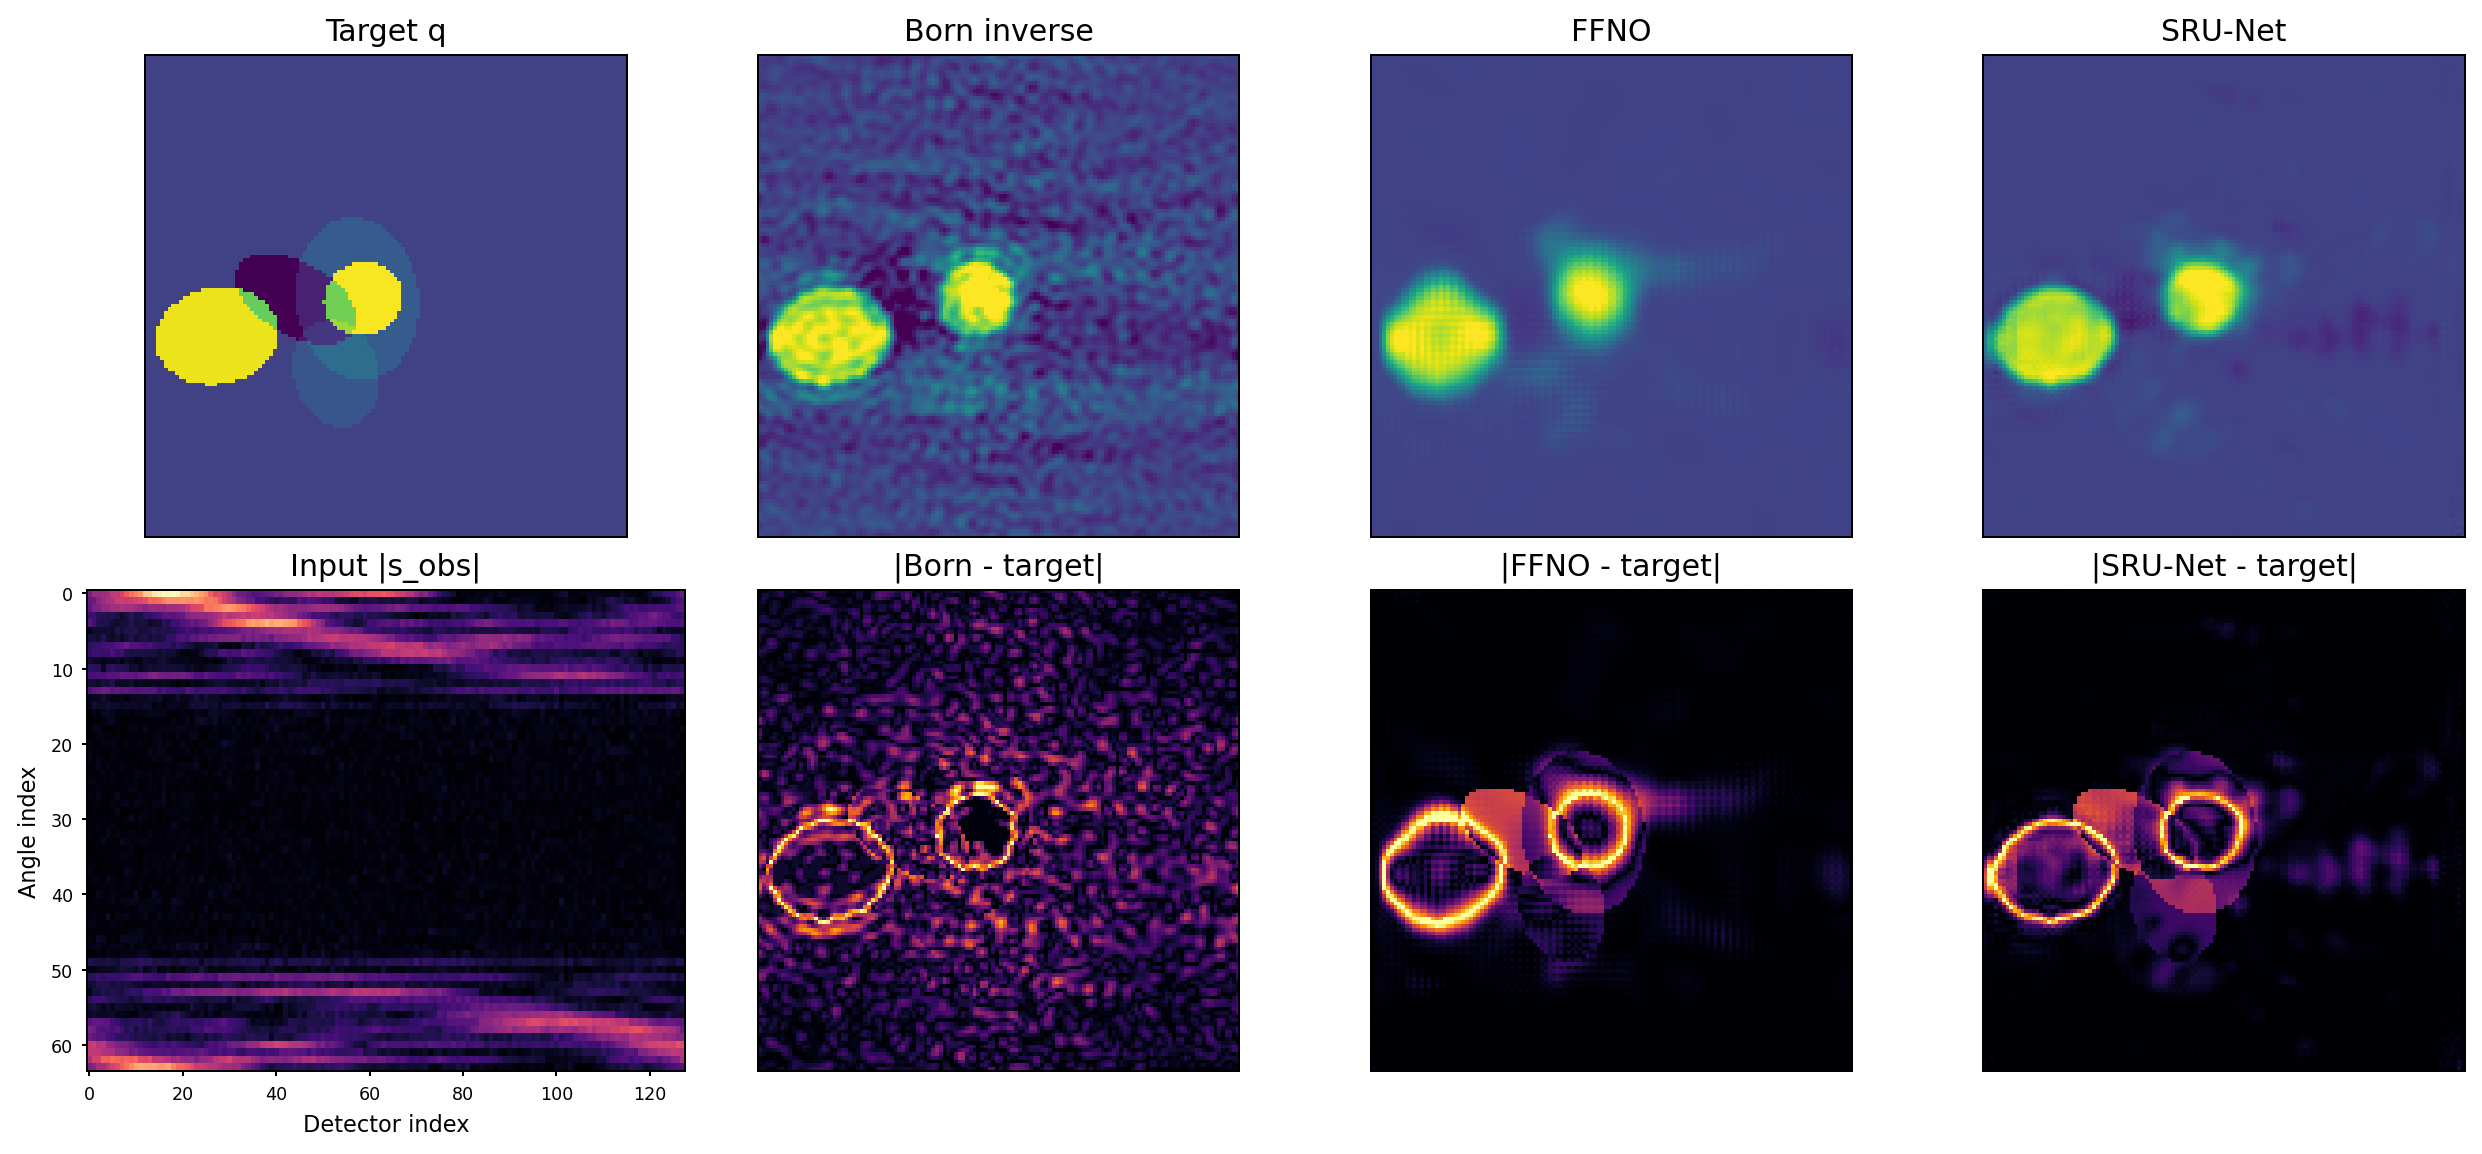
\includegraphics[width=\textwidth]{figures/brdt_sample_0255_context_recon_error.png}
\caption{\textbf{BRDT representative example.} The figure separates
the BRDT input $|s_{\mathrm{obs}}(\theta,d)|$ from the target scattering
potential $q$. The top row shows the target and three estimates
$\hat{q}$; the bottom row shows the input sinogram magnitude followed by
absolute target-domain errors under a shared error scale. The FFNO-labeled
panel is the historical local-refiner proxy, not the pending corrected
no-refiner BRDT FFNO rerun.}
\label{fig:brdt_candidate_recon}
\end{figure*}

\subsection{Secondary PDEBench CNS results}

Table~\ref{tab:cns_bundle} reports a single matched-condition CNS headline
ranking. All four rows share the same fixed contract:
\texttt{history\_len=5}, 512/64/64 train/validation/test trajectories,
40 training epochs, MSE loss, and identical optimizer and normalization
settings. FFNO gives the lowest aggregate and Fourier-band errors. SRU-Net$^*$
is the next strongest row by aggregate error and by high-frequency
\texttt{fRMSE}, with FNO third and U-Net behind on this capped slice. Because
this table uses a capped 512/64/64 split, we treat it as a matched-condition
architecture comparison rather than a full-training PDEBench benchmark.

% table_metadata: task=PDEBench_CNS; table_type=matched_condition_headline; selection_metric=err_nRMSE; history_len=5; data_split=train/val/test_trajectories=512/64/64; max_windows_per_trajectory=8; training_epochs=40; batch_size=4; training_loss=mse; claim_boundary=capped_matched_condition_comparison; source=docs/plans/NEURIPS-HYBRID-RESNET-2026/tables/pdebench_cns_matched_condition_metrics.tex; selection_authority=docs/plans/NEURIPS-HYBRID-RESNET-2026/pdebench_cns_matched_condition_table_refresh_summary.md
\begin{table}[t]
\centering
\scriptsize
\setlength{\tabcolsep}{3pt}
\caption{\textbf{PDEBench CNS matched-condition results.} All rows share the
\texttt{history\_len=5}, 512/64/64 train/validation/test split, 40-epoch capped
contract used for the head-to-head ranking. SRU-Net$^*$ denotes the
spectral-bottleneck SRU-Net variant. Low-, mid-, and high-band RMSE are
Fourier-band errors. Lower values are better. This is a bounded
matched-condition architecture comparison, not a full PDEBench state-of-the-art
claim.}
\label{tab:cns_bundle}
% Auto-generated CNS matched-condition headline table
\begin{tabular}{lrrrr}
\toprule
Model & nRMSE $\downarrow$ & Low RMSE $\downarrow$ & Mid RMSE $\downarrow$ & High RMSE $\downarrow$ \\
\midrule
FFNO & 0.0198 & 1.130 & 0.042 & 0.102 \\
SRU-Net$^*$ & 0.0331 & 1.854 & 0.171 & 0.262 \\
FNO & 0.0384 & 2.134 & 0.122 & 0.433 \\
U-Net & 0.5386 & 30.988 & 0.645 & 1.743 \\
\bottomrule
\end{tabular}

\end{table}

The CNS result is therefore bounded. It shows that SRU-Net transfers
competitively to a supervised forward-prediction setting and improves over FNO
and U-Net under this matched condition, but it does not establish SRU-Net as the
best CNS model. FFNO remains the lowest-error row in the CNS comparison.

% supplement_candidate: detailed CNS architecture, temporal-context, spectral-depth, Fourier-mode, convergence, and FFNO-local-feature tables preserved below for restoration or supplement migration. They are hidden from the main draft to keep the paper near the style-guide table budget.
\iffalse

\subsection{CNS architecture ablations}

The CNS secondary benchmark evaluates one architectural axis at a time while
keeping the data split, loss, and evaluation metrics unchanged. The first axis
is encoder-decoder fusion in the legacy hybrid shell: adding an additive skip
pathway lowers both aggregate and high-frequency error under the same training
budget.

% table_metadata: benchmark=PDEBench_CNS; cap_size=train_trajectories=512,val_trajectories=64,test_trajectories=64; window_counts=train=4096,val=512,test=512; full_split=train=8000,val=1000,test=1000; history_len=2; max_windows_per_trajectory=8; epochs=10; source=.artifacts/NEURIPS-HYBRID-RESNET-2026/phase-2-hybrid-skip-study/cns-skipadd-vs-base-10ep
\begin{table}[h]
\centering
\caption{Legacy hybrid shell ablation: additive encoder-decoder skip fusion.}
\begin{tabular}{lrr}
\toprule
Model & nRMSE & High-band RMSE \\
\midrule
Legacy hybrid shell baseline & 0.224425 & 1.243174 \\
Legacy hybrid shell with skip-add fusion & 0.104555 & 0.697058 \\
\bottomrule
\end{tabular}
\end{table}

The second axis is decoder upsampling. Holding the skip-fused architecture unchanged,
pixelshuffle gives the best aggregate error while avoiding the worst
high-frequency penalty of bilinear upsampling:

% table_metadata: benchmark=PDEBench_CNS; cap_size=train_trajectories=512,val_trajectories=64,test_trajectories=64; window_counts=train=4096,val=512,test=512; full_split=train=8000,val=1000,test=1000; history_len=2; max_windows_per_trajectory=8; epochs=10; source=.artifacts/NEURIPS-HYBRID-RESNET-2026/phase-2-hybrid-upsampler-artifact-study/cns-upsampler-cns-shell-10ep-20260421T221400Z
\begin{table}[h]
\centering
\caption{CNS spectral-convolutional upsampler comparison.}
\begin{tabular}{lrrr}
\toprule
Model & nRMSE & Relative $L_2$ & High-band RMSE \\
\midrule
Transpose upsampling & 0.130467 & 0.130467 & 0.763443 \\
Bilinear-convolution upsampling & 0.099081 & 0.099081 & 1.136333 \\
Pixelshuffle upsampling & 0.096320 & 0.096320 & 0.863959 \\
\bottomrule
\end{tabular}
\end{table}

Together, the skip-fusion and decoder ablations define the legacy hybrid
continuity row that is kept in metadata but not shown as a separate SRU-Net row
in the main CNS table.

\subsection{CNS temporal context}

Increasing CNS temporal context from two previous states to three previous
states improved the lower-error rows under the longer training budget:

% table_metadata: benchmark=PDEBench_CNS; cap_size=train_trajectories=512,val_trajectories=64,test_trajectories=64; window_counts=train=4096,val=512,test=512; full_split=train=8000,val=1000,test=1000; history_len=2_for_two-frame_columns,3_for_three-frame_columns; max_windows_per_trajectory=8; epochs=40; sources=history2 reference plus .artifacts/NEURIPS-HYBRID-RESNET-2026/phase-2-pdebench-cns-history-len3plus-compare/history3-pilot-40ep-20260429T073705Z; label_policy=SRU-Net* is the visible CNS label for repo row spectral_resnet_bottleneck_base; omitted_visible_row=hybrid_resnet_cns formerly shown as SRU-Net
\begin{table}[h]
\centering
\caption{CNS temporal-context comparison under the longer training budget.}
\begin{tabular}{lrrrr}
\toprule
Model & Two-frame nRMSE & Three-frame nRMSE & Two-frame high-band RMSE & Three-frame high-band RMSE \\
\midrule
SRU-Net$^*$ & 0.061562 & 0.045521 & 0.434933 & 0.346744 \\
% restore_if_needed: SRU-Net continuity row maps to repo row hybrid_resnet_cns; omitted CNS continuity row. Row values: SRU-Net & 0.064418 & 0.053843 & 0.368307 & 0.320036 \\
FNO & 0.074099 & 0.056725 & 0.671772 & 0.610477 \\
U-Net & 0.675798 & 0.677167 & 1.332625 & 1.173009 \\
\bottomrule
\end{tabular}
\end{table}

The result is consistent with the benchmark motivation: the task rewards models
that can use a longer coherent history, but the benefit is not uniform across
architectures or training budgets.

\subsection{CNS spectral depth and Fourier modes}

On the larger trajectory split, the shared spectral base model had lower
aggregate error, while the deeper shared-blocks10 row retained a small
mid/high-frequency edge at the same training budget:

% table_metadata: benchmark=PDEBench_CNS; cap_size=train_trajectories=1024,val_trajectories=128,test_trajectories=128; window_counts=train=8192,val=1024,test=1024; full_split=train=8000,val=1000,test=1000; history_len=2; max_windows_per_trajectory=8; epochs=40; label_policy=SRU-Net* is the visible CNS label for repo row spectral_resnet_bottleneck_base; source=.artifacts/NEURIPS-HYBRID-RESNET-2026/phase-2-pdebench-cns-hybrid-spectral-architecture-ablation/cns-hybrid-spectral-finalists-1024cap-40ep-20260428T054559Z
\begin{table}[h]
\centering
\caption{CNS spectral-depth comparison using 1024 training, 128 validation, and
128 test trajectories.}
\begin{tabular}{lrrrrrr}
\toprule
Model & nRMSE & RMSE & Low-band RMSE & Mid-band RMSE & High-band RMSE & Runtime (s) \\
\midrule
SRU-Net$^*$ & 0.043501 & 1.03746 & 2.4177 & 0.2224 & 0.2983 & 2162.70 \\
10-block shared-weight SRU-Net$^*$ & 0.044573 & 1.06304 & 2.4827 & 0.2168 & 0.2940 & 2703.72 \\
\bottomrule
\end{tabular}
\end{table}

A longer run showed that the earlier shared-blocks10 result had understated the
deeper profile:

% table_metadata: benchmark=PDEBench_CNS; cap_size=train_trajectories=1024,val_trajectories=128,test_trajectories=128; window_counts=train=8192,val=1024,test=1024; full_split=train=8000,val=1000,test=1000; history_len=2; max_windows_per_trajectory=8; epochs=40_and_80; label_policy=SRU-Net* is the visible CNS label for repo row spectral_resnet_bottleneck_base; sources=.artifacts/NEURIPS-HYBRID-RESNET-2026/phase-2-pdebench-cns-hybrid-spectral-architecture-ablation/cns-hybrid-spectral-finalists-1024cap-40ep-20260428T054559Z and .artifacts/NEURIPS-HYBRID-RESNET-2026/phase-2-pdebench-cns-shared-blocks10-1024cap-longer-convergence/cns-shared-blocks10-1024cap-80ep-20260429T025641Z
\begin{table}[h]
\centering
\caption{10-block shared-weight SRU-Net$^*$ under longer training on the larger
trajectory split.}
\begin{tabular}{lrrrrrr}
\toprule
Training epochs & nRMSE & RMSE & Low-band RMSE & Mid-band RMSE & High-band RMSE & Runtime (s) \\
\midrule
40 & 0.044573 & 1.06304 & 2.48274 & 0.216790 & 0.293987 & 2703.72 \\
80 & 0.037568 & 0.895959 & 2.10180 & 0.170457 & 0.215245 & 5364.49 \\
\bottomrule
\end{tabular}
\end{table}

The Fourier-mode studies show that simply increasing spectral modes is not a
clean default answer. Under the longer training budget, the 12-mode base model
retained better aggregate error, while 32/32 improved mid/high-frequency error:

% table_metadata: benchmark=PDEBench_CNS; cap_size=train_trajectories=512,val_trajectories=64,test_trajectories=64; window_counts=train=4096,val=512,test=512; full_split=train=8000,val=1000,test=1000; history_len=2; max_windows_per_trajectory=8; epochs=40; label_policy=SRU-Net* is the visible CNS label for repo row spectral_resnet_bottleneck_base; sources=spectral_resnet_bottleneck_base reference plus .artifacts/NEURIPS-HYBRID-RESNET-2026/phase-2-pdebench-cns-spectral-modes32-compare/cns-spectral-modes32-40ep-20260428T014353Z
\begin{table}[h]
\centering
\caption{CNS Fourier-mode comparison under the longer training budget.}
\begin{tabular}{lrrrrrr}
\toprule
Model & nRMSE & RMSE & Mid-band RMSE & High-band RMSE & Params & Runtime (s) \\
\midrule
SRU-Net$^*$, 12 modes & 0.061562 & 1.48776 & 0.2800 & 0.4349 & 8,186,726 & 1861.63 \\
SRU-Net$^*$, 32 modes & 0.064551 & 1.55999 & 0.2425 & 0.3472 & 42,388,614 & 1382.12 \\
\bottomrule
\end{tabular}
\end{table}

In the 24-mode comparison with still longer training, the shared 12-mode base
model was ahead on every reported metric, but both models were still improving
according to the convergence audit:

% table_metadata: benchmark=PDEBench_CNS; cap_size=train_trajectories=1024,val_trajectories=128,test_trajectories=128; window_counts=train=8192,val=1024,test=1024; full_split=train=8000,val=1000,test=1000; history_len=2; max_windows_per_trajectory=8; epochs=80; label_policy=SRU-Net* is the visible CNS label for repo row spectral_resnet_bottleneck_base; source=.artifacts/NEURIPS-HYBRID-RESNET-2026/phase-2-pdebench-cns-spectral-modes24-convergence-compare/cns-spectral-modes24-vs-base-1024cap-80ep
\begin{table}[h]
\centering
\caption{CNS 12-mode versus 24-mode spectral comparison under still longer
training.}
\begin{tabular}{lrrrrrr}
\toprule
Model & nRMSE & RMSE & Low-band RMSE & Mid-band RMSE & High-band RMSE & Params \\
\midrule
SRU-Net$^*$, 12 modes & 0.038269 & 0.912674 & 2.11528 & 0.220081 & 0.282737 & 8,391,814 \\
SRU-Net$^*$, 24 modes & 0.039533 & 0.942819 & 2.17721 & 0.241145 & 0.306903 & 25,152,646 \\
\bottomrule
\end{tabular}
\end{table}

Together these results support the architecture thesis: more spectral capacity
can help selected high-frequency quantities, but useful performance depends on
local paths, decoder behavior, convergence, and parameter cost.

\subsection{CNS FFNO local features}

Adding an explicit local-convolution branch to the in-repository FFNO-style
bottleneck improved both aggregate and high-frequency metrics:

% table_metadata: benchmark=PDEBench_CNS; cap_size=train_trajectories=512,val_trajectories=64,test_trajectories=64; window_counts=train=4096,val=512,test=512; full_split=train=8000,val=1000,test=1000; history_len=2; max_windows_per_trajectory=8; epochs=40; sources=.artifacts/NEURIPS-HYBRID-RESNET-2026/phase-2-pdebench-ffno-convolutional-features-cns/cns-ffno-close-backfill-40ep-20260428T084852Z,.artifacts/NEURIPS-HYBRID-RESNET-2026/phase-2-pdebench-ffno-convolutional-features-cns/cns-ffno-localconv-40ep-20260428T090626Z,.artifacts/NEURIPS-HYBRID-RESNET-2026/phase-2-pdebench-author-ffno-equal-footing-cns/author-ffno-40ep-20260422T234340Z
\begin{table}[h]
\centering
\caption{CNS FFNO-family local-convolution comparison under the longer training
budget.}
\begin{tabular}{lrrrr}
\toprule
Model & Relative $L_2$ & High-band RMSE & Params & Runtime (s) \\
\midrule
FFNO bottleneck & 0.076224 & 0.3934 & 6,809,701 & 980.52 \\
FFNO + local conv & 0.055773 & 0.3091 & 7,695,205 & 1031.22 \\
Reference FFNO & 0.028148 & 0.1210 & 1,073,672 & 4725.51 \\
\bottomrule
\end{tabular}
\end{table}

The local-convolution branch improves the local FFNO-family proxy, but the
reference FFNO remains the lower-error row under the same CNS comparison. Within
the no-external-data CNS experiments reported here, reference FFNO is the
lowest-error observed non-pretrained neural-operator baseline. This is
consistent with the original F-FNO motivation of improving FNO accuracy and
scaling on PDE benchmarks, including Navier-Stokes-style
settings~\cite{ffno,pdebench}.

\fi

\section{Discussion}

The main finding is that physics-consistent wave inverse reconstruction depends
on both the objective and the architecture. In the synthetic CDI controls,
direct supervised object-space training is not interchangeable with training
through the known diffraction model. Where paired rows are available,
supervised training can produce poor or unbalanced amplitude--phase
reconstructions, while physics-consistency training gives stronger
measurement-consistent reconstruction behavior. The CDI loss is therefore not
an incidental training detail in this benchmark.

The second finding is that the physics-consistency objective does not remove the
need for an appropriate inverse architecture. SRU-Net encodes the global-local
structure of the task directly: Fourier-style encoder branches provide global
mixing, local convolutional branches preserve grid-aligned detail, the residual
bottleneck refines features at reduced spatial resolution, and the decoder
synthesizes the real-space output. The CDI architecture comparison and
spectral-component ablations show that performance depends on where spectral
coupling is introduced and how it is paired with local convolutional paths,
residual refinement, and decoder-side upsampling. Adding spectral capacity alone
does not reproduce the SRU-Net result.

The evidence should be interpreted narrowly. The primary claim is about
synthetic CDI wave inverse reconstruction under the stated $N=128$ protocol.
The objective controls are paired only for the architectures where both
supervised and physics-informed rows are available, so claims about supervised
failure should be limited to those controls unless additional paired rows are
added. The current FFNO-local proxy rows include local CNN refinement and should
not be used as canonical pure-FFNO baselines.

The secondary experiments provide context rather than the central claim. BRDT
shows bounded transfer to a second wave inverse problem, but the reported FFNO
comparison is a historical local-refiner proxy pending corrected no-refiner
runs. PDEBench CNS shows that SRU-Net is competitive with FNO and U-Net under a
matched capped condition, but FFNO remains the lowest-error CNS model. The CNS
results therefore support the global-local architectural motivation without
claiming PDEBench state-of-the-art performance.

\iffalse
\section{Additional Experiments}

\subsection{Hybrid skip/residual ablation}

% table_metadata: task=CDI_lines128; ablation=hybrid_skip_residual; authority=architecture_ablation; source=.artifacts/work/NEURIPS-HYBRID-RESNET-2026/backlog/2026-04-30-cdi-lines128-hybrid-resnet-skip-residual-ablation
\begin{table}[t]
\centering
\small
\caption{\textbf{Hybrid skip/residual ablation on synthetic CDI.} Rows vary
skip-fusion and residual-scale choices under the same $N=128$ protocol. MAE
denotes mean absolute error, and FRC50 denotes the Fourier-ring-correlation
0.5-crossing metric; lower MAE and higher FRC50 are better.}
\label{tab:cdi_skip_residual_ablation}
\begin{tabular}{lrrrr}
\toprule
Variant & Amplitude MAE $\downarrow$ & Phase MAE $\downarrow$ &
Amplitude FRC50 $\uparrow$ & Phase FRC50 $\uparrow$ \\
\midrule
SRU-Net (reference) & 0.0269 & 0.0721 & 135.46 & 106.80 \\
skip-add & 0.0264 & \textbf{0.0610} & 135.39 & \textbf{135.96} \\
fixed residual scale & \textbf{0.0246} & 0.0773 & \textbf{135.92} & 106.68 \\
skip-add + fixed residual & 0.0289 & 0.0633 & 135.41 & 106.88 \\
\bottomrule
\end{tabular}
\end{table}

Skip-add is the clearest phase-oriented variant, while fixed residual scaling is
the clearest amplitude-oriented variant. Combining the two did not produce a
constructive interaction in this small same-protocol ablation.
\fi

\clearpage
\appendix

\section{BRDT FNO Objective Control}

% figure_metadata: task=BRDT; source_supervised=.artifacts/NEURIPS-HYBRID-RESNET-2026/backlog/2026-04-29-brdt-four-row-preflight/figures/source_arrays/sample_0255_fno_vanilla_*; source_physics_only=.artifacts/NEURIPS-HYBRID-RESNET-2026/backlog/2026-05-04-brdt-physics-only-objective-ablation/figures/source_arrays/sample_0255_fno_vanilla_*; paper_copy=figures/brdt_fno_objective_ablation.png; role=appendix_objective_control
\begin{figure*}[t]
\centering
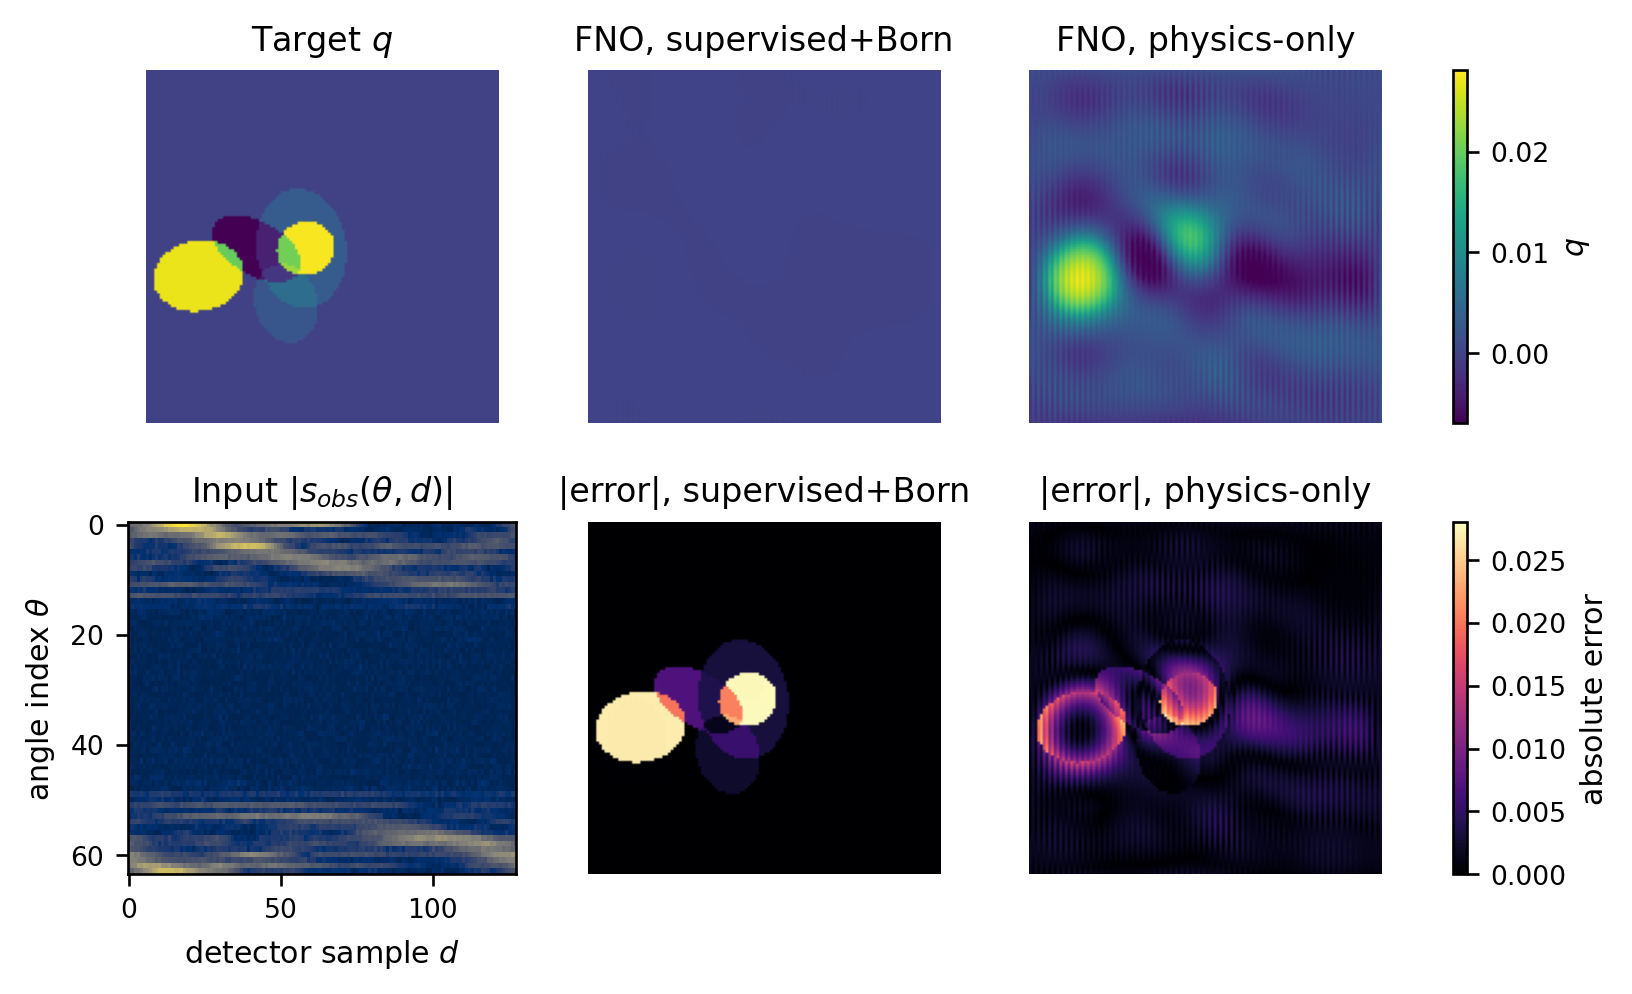
\includegraphics[width=\textwidth]{figures/brdt_fno_objective_ablation.png}
\caption{\textbf{BRDT FNO objective control.} Vanilla FNO did not converge
under the supervised object loss plus Born-consistency objective used for the
main BRDT comparison, producing a nearly constant reconstruction. Under a
physics-only objective on the same BRDT split and representative example, the
same architecture recovers visible object structure. This control is therefore
reported separately from Fig.~\ref{fig:brdt_candidate_recon}, whose columns
remain a controlled comparison of the reported BRDT rows.}
\label{fig:brdt_fno_objective_ablation}
\end{figure*}

\section{CNS Adjacent-Context Visualization}

% figure_metadata: task=PDEBench_CNS; train_trajectories=512; val_trajectories=64; test_trajectories=64; fixed_sample=0; visible_rows=target,author_ffno_cns_base,spectral_resnet_bottleneck_base,fno_base,unet_strong; omitted_row=hybrid_resnet_cns; fields=density,pressure; panels=prediction_and_abs_error; label_policy=SRU-Net* is the visible CNS label for repo row spectral_resnet_bottleneck_base; figure_role=adjacent_context_only; figure_lane=h2_512_64_64_2step; source=.artifacts/NEURIPS-HYBRID-RESNET-2026/backlog/2026-04-29-cns-paper-table-figure-bundle/figures/sample000
% restore_if_needed: omitted CNS figure column maps visible label SRU-Net to repo row hybrid_resnet_cns. Source panels: density__hybrid_resnet_cns__prediction.png, density__hybrid_resnet_cns__abs_error.png, Vx__hybrid_resnet_cns__prediction.png, Vx__hybrid_resnet_cns__abs_error.png, Vy__hybrid_resnet_cns__prediction.png, Vy__hybrid_resnet_cns__abs_error.png, pressure__hybrid_resnet_cns__prediction.png, pressure__hybrid_resnet_cns__abs_error.png.
\begin{figure}[h]
\centering
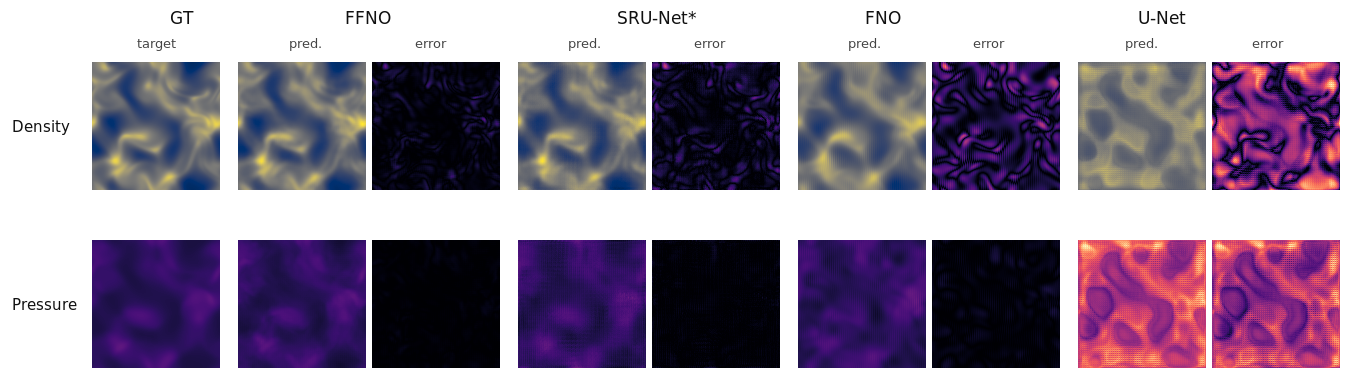
\includegraphics[width=\linewidth]{figures/pdebench_cns_sample000_predictions.png}
\caption{\textbf{PDEBench CNS fixed-sample predictions and errors
(adjacent context).} The shared test sample comes from the earlier
2-input-time-step 512/64/64 CNS visual comparison and is shown only as
adjacent-context illustration of per-row error structure. The
matched-condition headline ranking in Table~\ref{tab:cns_bundle} uses the
\texttt{history\_len=5} contract; this figure is not the same-condition
fixed-sample comparison for that contract.}
\label{fig:cns_sample_predictions}
\end{figure}

\section{Secondary CNS Follow-Up Comparisons}

Table~\ref{tab:cns_ablation} reports selected SRU-Net$^*$ follow-up comparisons
on CNS. These rows are not used as the main ranking table. They show how
temporal context, retained Fourier modes, and bottleneck depth affect aggregate
and Fourier-band errors under bounded training budgets. The results support the
architectural interpretation that spectral capacity alone is not a universal
solution; useful performance depends on temporal context, local paths, decoder
behavior, convergence, and parameter cost.

% table_metadata: task=PDEBench_CNS; ablation=SRU-Net_components; source=multiple existing bounded CNS studies; detailed source rows preserved in supplement_candidate block below
\begin{table}[t]
\centering
\scriptsize
\setlength{\tabcolsep}{3pt}
\caption{\textbf{Selected SRU-Net$^*$ follow-up comparisons on PDEBench CNS.}
SRU-Net$^*$ denotes the spectral-bottleneck SRU-Net variant. The ablation axis
is the architectural or input-context change named in the first column; the
second column records run context only. All rows use 40 training epochs. Low-,
mid-, and high-band RMSE are Fourier-band errors. Lower values are better.}
\label{tab:cns_ablation}
\begin{tabular}{p{1.18in}p{1.45in}rrrr}
\toprule
Tested axis & Run context & nRMSE $\downarrow$ &
Low RMSE $\downarrow$ & Mid RMSE $\downarrow$ & High RMSE $\downarrow$ \\
\midrule
Reference setting & 512/64/64 split; 2 input steps & 0.062 & 3.476 & 0.280 & 0.435 \\
% restore_if_needed: SRU-Net continuity row maps to repo row hybrid_resnet_cns; omitted CNS continuity row. Row values: SRU-Net, two-frame & 512/64/64, 40ep & 0.064 & 0.368 \\
Longer temporal context & 512/64/64 split; 3 input steps & 0.046 & 2.560 & 0.216 & 0.347 \\
More retained Fourier modes & 512/64/64 split; 2 input steps & 0.065 & 3.676 & 0.242 & 0.347 \\
Deeper shared-weight spectral bottleneck & 1024/128/128 split; 2 input steps & 0.045 & 2.483 & 0.217 & 0.294 \\
\bottomrule
\end{tabular}
\end{table}

\section{Model Configurations}

\begin{table*}[t]
\centering
\scriptsize
\setlength{\tabcolsep}{3pt}
\caption{\textbf{Model configurations by benchmark.} Parameter counts are
unique trainable parameters in the effective prediction model. Wrapper
state-dict counts are not used when they duplicate the same generator under
multiple aliases.}
\label{tab:model_config_by_benchmark}
\resizebox{\textwidth}{!}{\begin{tabular}{lllrrrrll}
\toprule
Benchmark & Model & Training & Width & Modes & Enc. & Bott. & Down & Unique params \\
\midrule
Synthetic CDI & CNN & physics-consistency & -- & -- & -- & -- & -- & 4,661,212 \\
Synthetic CDI & FNO & physics-consistency & 32 & 12 & 4 & -- & -- & 636,450 \\
Synthetic CDI & FFNO (pinn\_ffno) & physics-consistency & 32 & 12 & 4 & -- & -- & 124,966 \\
Synthetic CDI & SRU-Net & physics-consistency & 32 & 12 & 4 & 6 & 2 & 9,003,299 \\
Synthetic CDI & U-NO & physics-consistency & 32 & 12 & 4 & -- & -- & 1,257,858 \\
Synthetic CDI & CNN & supervised & -- & -- & -- & -- & -- & 4,612,418 \\
Synthetic CDI & FFNO (supervised\_ffno) & supervised & 32 & 12 & 4 & -- & -- & 124,966 \\
Synthetic CDI & U-NO & supervised & 32 & 12 & 4 & -- & -- & 1,257,858 \\
\midrule
PDEBench CNS & FFNO & supervised & 64 & 16 & 24 & -- & -- & 1,074,440 \\
PDEBench CNS & SRU-Net & supervised & 32 & 12 & 4 & 6 & 2 & 8,395,270 \\
PDEBench CNS & FNO & supervised & 32 & 12 & 4 & -- & -- & 358,628 \\
PDEBench CNS & U-NO & supervised & 32 & 12 & 4 & -- & -- & 1,260,548 \\
PDEBench CNS & U-Net & supervised & 32 & -- & -- & -- & -- & 7,768,036 \\
\midrule
BRDT & SRU-Net & supervised + Born & 16 & 8 & 2 & 2 & 1 & 142,018 \\
BRDT & FFNO & supervised + Born & 16 & 8 & 4 & -- & -- & 27,394 \\
\bottomrule
\end{tabular}
}
\end{table*}

\begin{thebibliography}{9}

\bibitem{hoidn2023physics}
Oliver Hoidn, Aashwin Ananda Mishra, and Apurva Mehta.
\newblock Physics constrained unsupervised deep learning for rapid, high
resolution scanning coherent diffraction reconstruction.
\newblock \emph{Scientific Reports}, 13:22789, 2023.
\newblock \url{https://www.nature.com/articles/s41598-023-48351-7}.

\bibitem{fno}
Zongyi Li, Nikola Kovachki, Kamyar Azizzadenesheli, Burigede Liu,
Kaushik Bhattacharya, Andrew Stuart, and Anima Anandkumar.
\newblock Fourier neural operator for parametric partial differential equations.
\newblock \emph{International Conference on Learning Representations}, 2021.
\newblock \url{https://arxiv.org/abs/2010.08895}.

\bibitem{localno}
Miguel Liu-Schiaffini, Julius Berner, Boris Bonev, Thorsten Kurth,
Kamyar Azizzadenesheli, and Anima Anandkumar.
\newblock Neural operators with localized integral and differential kernels.
\newblock \emph{International Conference on Machine Learning}, 2024.
\newblock \url{https://arxiv.org/abs/2402.16845}.

\bibitem{ufno}
Gege Wen, Zongyi Li, Kamyar Azizzadenesheli, Anima Anandkumar, and
Sally M. Benson.
\newblock U-FNO -- an enhanced Fourier neural operator-based deep-learning
model for multiphase flow.
\newblock \emph{Advances in Water Resources}, 163:104180, 2022.
\newblock \url{https://doi.org/10.1016/j.advwatres.2022.104180}.

\bibitem{ffno}
Alasdair Tran, Alexander Mathews, Lexing Xie, and Cheng Soon Ong.
\newblock Factorized Fourier neural operators.
\newblock \emph{International Conference on Learning Representations}, 2023.
\newblock \url{https://arxiv.org/abs/2111.13802}.

\bibitem{pdebench}
Makoto Takamoto, Timothy Praditia, Raphael Leiteritz, Daniel MacKinlay,
Francesco Alesiani, Dirk Pflueger, and Mathias Niepert.
\newblock PDEBench: An extensive benchmark for scientific machine learning.
\newblock \emph{Advances in Neural Information Processing Systems}, 2022.
\newblock \url{https://arxiv.org/abs/2210.07182}.

\end{thebibliography}

\end{document}
